% !TEX root = arbeit.tex
\section{Experiments} \label{sec:Exp}
	The tests described in this chapter include tests of the different components of the NIM instrument such as laboratory tests of the flight antechamber tested on the Prototype or the flight ion-mirror. The part of Chapter \ref{sec:Exp} includes manly test with the prototype, later on tests with the PFM and follow.

% In zeitlicher Reihenfolgen auflisten, damit man sieht, zu welchem Zeitpunkt man mit welchen Teilen gearbeitet hat.
% In this section, all the different test (lab and simulations) are listed. As far as possible in their chronolocial order because between some lab tests there were simulations to improve the instrument before testing the redesigned instrument.

% Fügt ein PDF ein, nummeriert nach dem PDF normal weiter.
%\includepdf[pages=-]{Report_Thermofoil_UV_Masterarbeit.pdf}

% Section über Detector? haben wir ja nicht wirklich etwas gemacht. Diode durch 2 Widerstände ersetzt. -> Spannungsfestigkeit. Verlauf der Überschläge. Unterschiedliche Skizzen.

	In this section, the different tests are described to develop the NIM instrument. Different parts of the instrument were tested to improve the instrument.
%-----------------------------------------------------------------------------------
	\subsection{Ion-Mirror}
	% Test of subcomponents.
	The NIM prototype reflectron was exchanged through the flight like reflectron, which was tested. The NIM prototype reflectron consisted of 12 ring electrodes connected with each other with resistors in between them. On the first, 5th and 12th electrode, a voltage can be applied. With the different resistors, a linear voltage gradient in the reflectron is generated.\\ % Noch besser formulieren.
	The flight reflectron consists of a ceramic tube with two resistance spirals on its inner walls. There are three electrodes, where the voltage can be applied. The electrodes are connected via resistance spirals with each other. The two reflectrons can be seen in Fig.\,\ref{fig:ExpRefl}. This kind of reflectron was also used in the RTOF mass spectrometer which flied in ROSINA \cite{Diss_Scherer} and the in the NGMS \cite{Diss_Hofer}. \\ % Evt. noch etwas schöner und weiter ausführen. Strahlungsfestigkeit musste getestet werden. Report? Paper? Diss?
	Therefore, the two reflectrons are from the electrical point of view the same.\\ % Oder kommt das erst bei der Auswertung?
	
	\begin{figure}[h]
		\begin{subfigure}{0.5\textwidth}
			\centering
			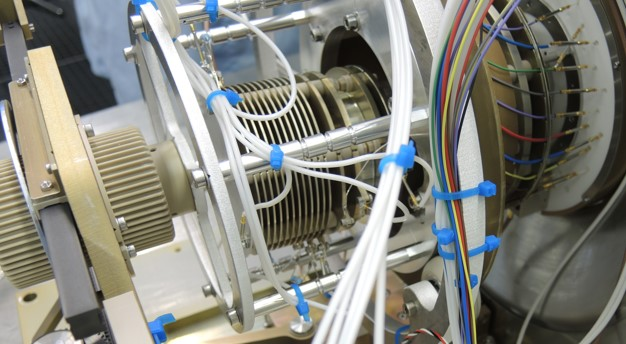
\includegraphics[width = 0.95\textwidth]{Experiments/reflectron_Prototype1.jpg}
		\end{subfigure}
		\begin{subfigure}{0.5\textwidth}
			\centering
			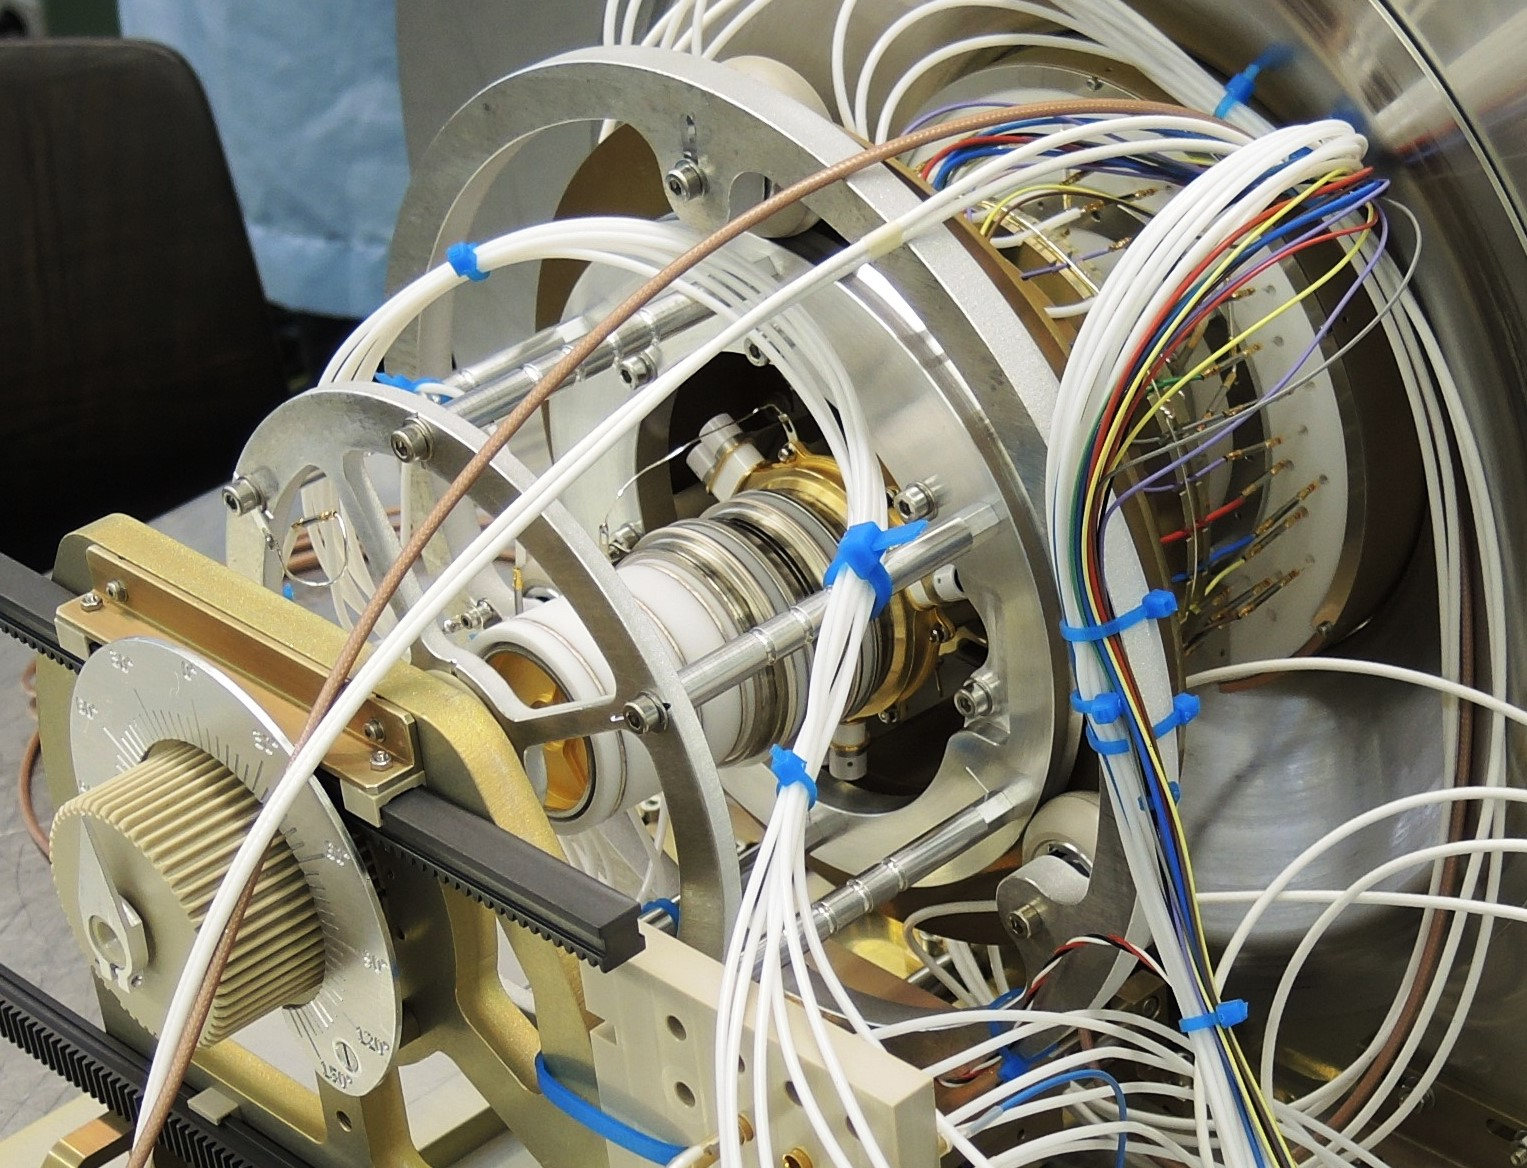
\includegraphics[width = 0.85\textwidth]{Experiments/reflectron_flight.JPG}
		\end{subfigure}
		\caption{Left: Prototype reflectron with ringelectrodes. Right: Flight reflectron}
		\label{fig:ExpRefl}
	\end{figure}

	\subsubsection{Measurement Principle}\label{subsec:ReflecMeasPric}
		% Vortrag Messbedingungen zusammenschreiben
	
	\subsubsection{Discussion}\label{subsec:ReflecDissc}
		% Graphiken neu machen. Achsenskalierung, Spannungssets-Vergleich? Nur sagen, dass sie beinahe identisch sind.
	
	
	% Messbedingungen. Eigenes kurzes Unterkapitel machen
	% Auswertung, eigenes kurzes Unterkapitel

	\begin{comment}
	
	Exchange of the reflectron. Messdaten und Auswertung. Spannungssets vergleichen. Vortrag zusammenschreiben. Plots von dort nehmen und noch etwas besser beschreiben.
	(Plot-Axis, enlarge the exponent of the 10^11 e-/ns)
						
	\end{comment}
	
	
	
	\subsection{Prototype CASYMIR-D/-E}
	% CASYMIR-D? Erst wenn man intensitätsproblem mit ante chamber gelöst hat :/. CASYMIR-E-Kampagne.
	% Kurzfassung?
	
%--------------------------------------------------------------------------------
	\subsection{Simulations}
	
	During development, the mounting of the HV lenses was adapted. Simulations had to be done because as a result of the changed form of the lenses, the voltage set also changed. In this case, the voltage ranges increase by about blabla volts. These new higher ranges challenged the design of the supply electronics because the electronics has a limited amount of space. % Look up the details. Explanation with the electric fields?
	
	%\textcolor{red}{\textbf{Simulations of the adaption of the mounting of the electrodes has to come before the experiments with the PFM although the PFM structure is explained before.}}
	
	% Maybe an other arrangement of the Simulations chaper. See whicht simulations are performed how far any in which order they have to be to be comprehendible.
	
	% Evt. in einem eigenen Kapitel? Schauen, welchen Einfluss es dann jeweis auf die Hardware hatte. -> Elektronik setzt Spannungsranges, beschreiben, dass man da iterieren musste um das optimale Simulationsspannungsset zu finden mit den Grenzen, welche die Elektronik uns für die jeweiligen Elektroden gibt. -> vgl. mit den Messungen vom PFM.
	% Neusimulationen mit neuen Grenzen für die HV. -> die Resultate dieser Simulationen. Als Folgen davon wurden die Grenzen für die HV neu definiert. Schauen, wie man das am besten auseinander nimmt :/.

	% Change of the mounting of the IS lenses -> change in voltages

	% Pulsersimulationen -> Kriterien für Andy für das Pulserdesign. Ab wann wir einen Einbruch in der Massenauflösung haben. (Worddokument wo die einzelnen Bilder zusammengestellt sind?)
	
	% Filament repeller simulation tests. Noch Graphiken einmal einfügen. Die wichtigsten.
	% Um herauszufinden, wie wichtig die Position des Filaments ist.
	
	% Noch besser umschreiben. Die position des filaments entspricht nicht der erwarteten??? Was ist da schief gelaufen??? :(
	
	% Intensitätssimulation Countberechnung:
	% Man generiert 2000 e- auf dem Filament und zeichnet immer nach 1E-5 microsec auf, an welcher Position sich die Teilchen gerade befinden. Die Fkt. 'Plot_optVoltAndPos.m' zählt alle Positionen zusammen, welche sich in dem Zylindervolumen befinden. Die Grundfläche des Zylinders ist das Eintritts-Grid von der antechamber und die Höhe ist die Höhe der Entrance. Im th-Mode befinden sich nur in diesem Volumen neutrale Teilchen.
	\begin{figure}[h]
		\begin{subfigure}{0.53\textwidth}
			\centering
			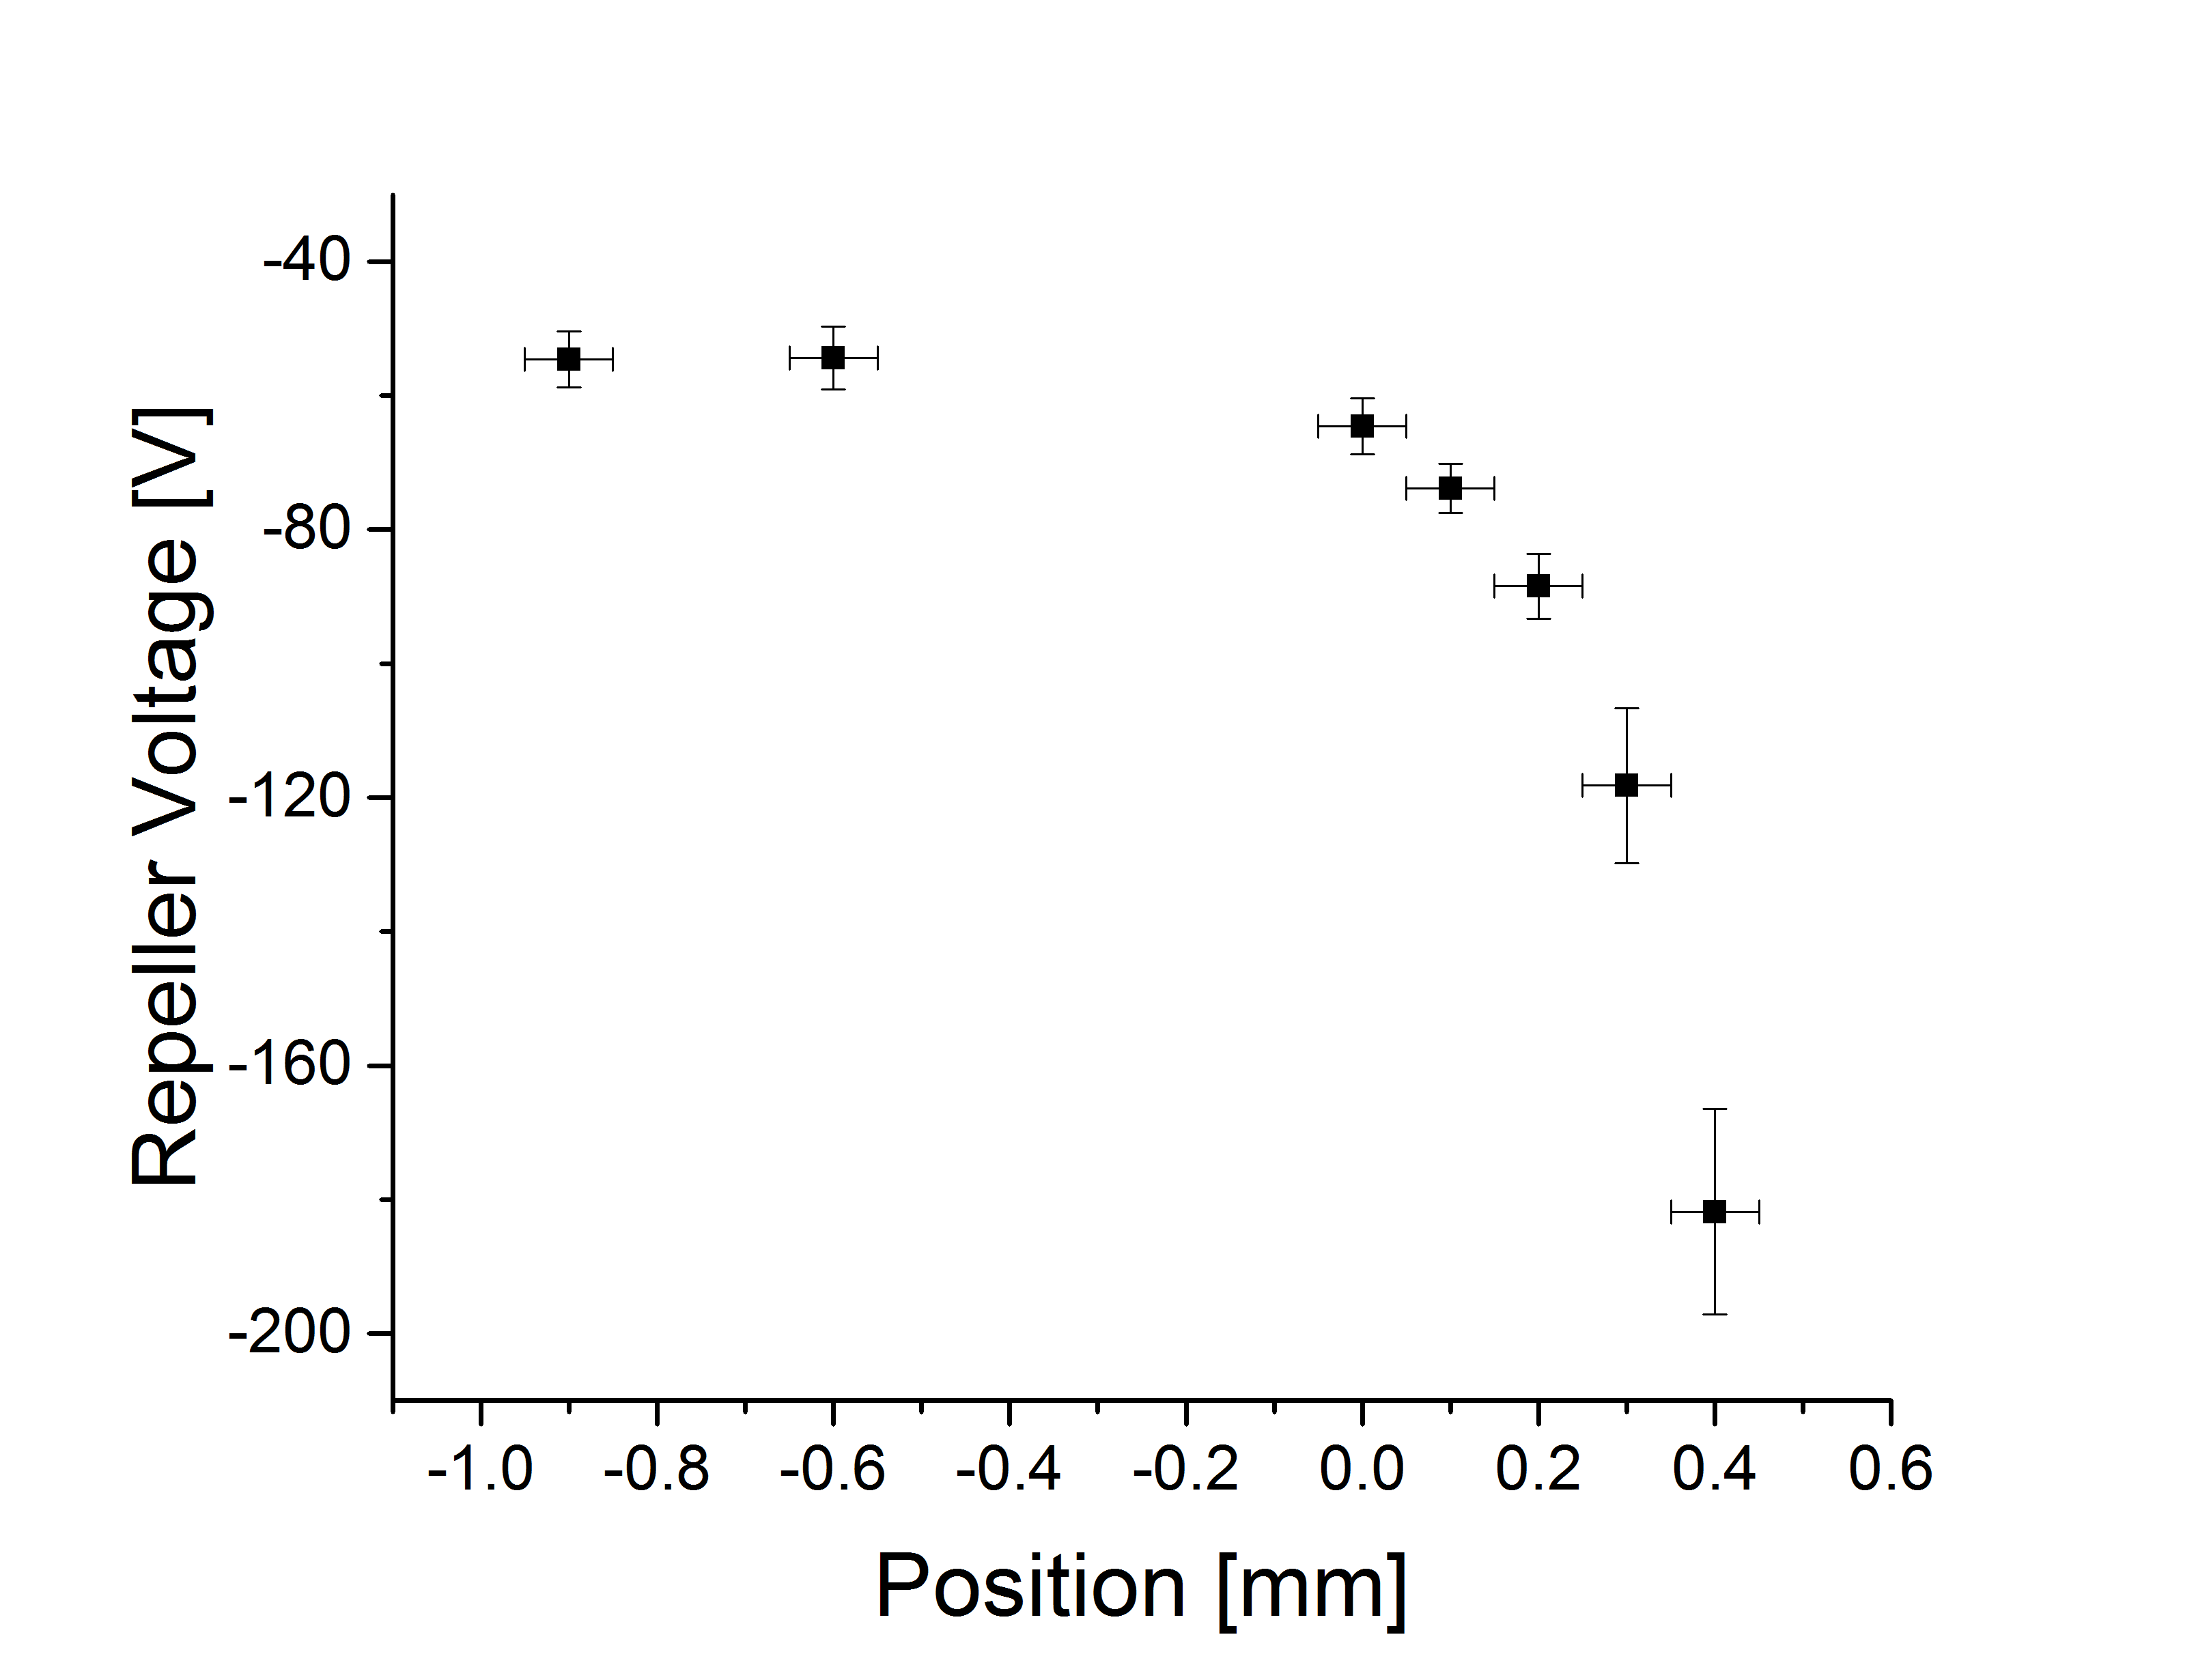
\includegraphics[width= 0.95\textwidth]{Experiments/SimRepPosU.png}
		\end{subfigure}
		\begin{subfigure}{0.47\textwidth}
			\centering
			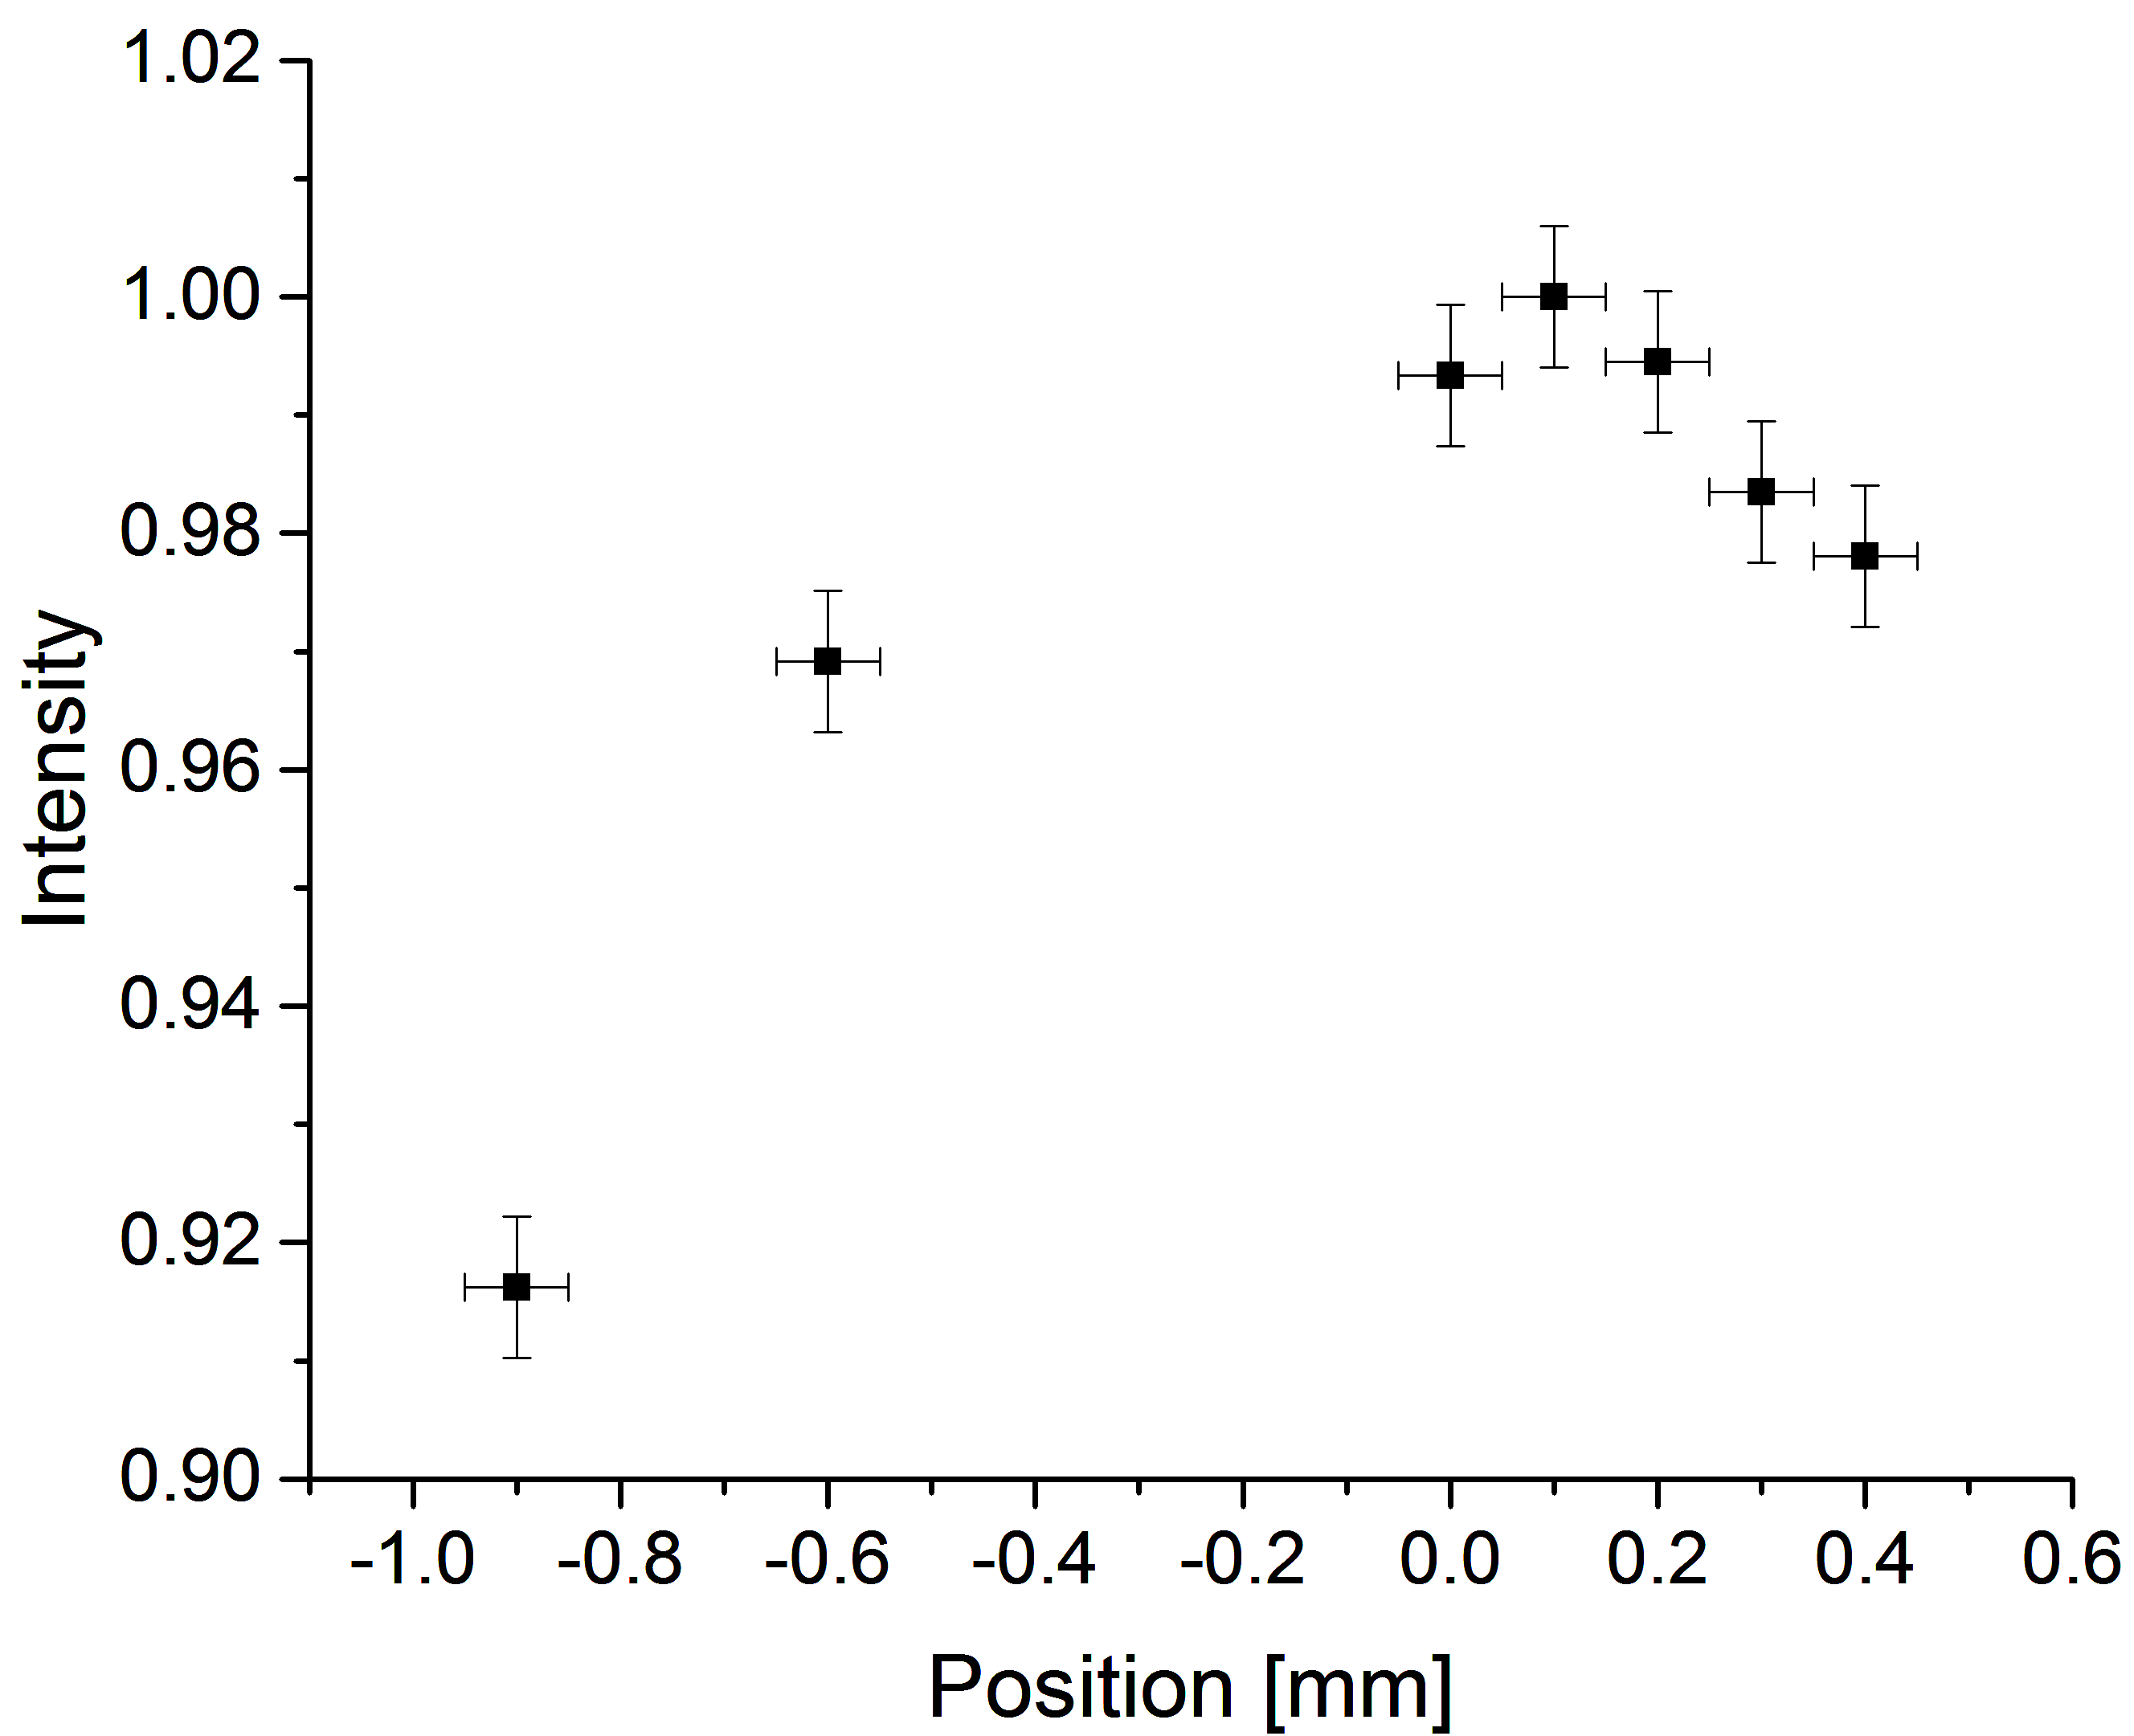
\includegraphics[width= 0.95\textwidth]{Experiments/SimRepPosImax.png}
		\end{subfigure}
		\caption{Left: The filament repeller voltage to reach the maximum electron intensity over the volume of the neutral particles. Right: Electron intensity normed on the intensity at position 0.} % Noch Graphik wie Intensität bei den versch. Pos abfällt.
		\label{fig:ExpSimRep}
	\end{figure}

	\subsection{Filament decision}
	% Ranking criterion -> Explanation, see electronics book. constant power of one filament -> resistance variies over time. Vgl. Diss Rico.

%------------------------------------------------------------------------------------
	\subsection{Pulser}
	% Simulations with different rise times and their influence on the mass spectrum.
	% Test with lab pulser, wavelab pulser -> compare their properties and their performance.
	
	% Pulsertests, Messungen, Simulationsresultate
	% Two different pulsers properties, pulse shape. Tests with different gases. Massresolution, Intensity relation?, SNR? Are these two properties correlated? Noch mit Peter anschauen. Ar sieht in allen 4 Fällen etwas komisch aus. Higher signal intensity -> higher SNR.
	% Achsenskalierung anschauen von Areagraphik. Wenn das geklärt ist, evt. in Matlab schreiben. Zusätzliches Skript für diese Graphiken, Stefans Vorlagen anschauen. Die signal intensity lässt sich nicht einfach in Druck umrechnen. Zu viele unbekannte Komponenten -> a.u. oder # e-/ns angeben.
	
	
	
	\subsection{Detector Tests}
	% FS IsoArea. Variation of the MCP gain an observation how the SNR and IsoArea change. \\titania.unibe.ch\UserHomes\foehn\MyDocuments\PhD\Messungen\FS\ firstOpti\MCP_Gain.opj
	% Also show different signal heights/ forms? Defect diode, functioning diode, resistor? Full gain curve is only possible for functioning diode (tests to be done) and resistor (plot already included).
	The following chapter describes improvements of the mechanical and electrical design of the NIM PFM detector and tests performed with different versions. Most of the tests were performed in the Pumpstand nr.2 (Chapter \ref{subsubsec:SetFacPumpst}) and a few were done with the detector in the sensor Proto Flight Model (PFM) or in the sensor flight spare model (FS).\\
	% Leave this part here as it is a description of the process we were working on. Describe the adaption of the meachanical design of the detector housing, the consequence that we inserted a resistor instead of an anode. Pros and Cons of the Anode vs. the resistor?
	% Description of the housing and problems related to it -> investigation, improvements.
	The detector suffered repeatedly discharges causing a failure of the diode, which is one of the key components of the detector. This lead to a redesign of the detector housing and to an exchange of the diode through a resistor, because the resistor is more robust concerning discharges. % Include an electrical schema. May a zoom of the other one laready included in the setup chapter (as soon as it is finished). Explanation about how a diode works? Talk with JoGa maybe. Explain main hypothesis why it died repeatedly?
	The discharges could be eliminated by a redesign of the detector housing. % Vgl. Fig. of the 2 housing designs (start and end) and explain them.
	Fig.bla left shows an earlier version of the detector housing and Fig. bla right shows the design of the current flight detector.
	Basically, the MCPs lay on a border about 1 mm above the anode. % Check distance
	A diode generates an additional voltage difference between the MCP backside and the anode to accelerate the electrons from the MCP backside towards the anode. Between this border and the MCP is the contact lug which is connected to the high voltage rail. On top of the upper MCP is the contact lug to connected to the corresponding voltage rail. On top of that is a bushing and a sort of screw. When tightening the screw, the bushing presses uniformly on the MCPs. In the old design, the thread for the screw was cut down to the boarder on which the MCPs lay. When assembling the whole stack, the MCPs often cant in the thread. Another challenge lay in tightening of the screw. When the screw was too loose, the top and the bottom contact lug had no reliable contact to the MCPs. When applying a high voltage over the whole MCP stack, the gap acts as an additional resistor over which the voltage build up resulting in a discharge between the corresponding electrode and the MCP. The discharge can propagate through the whole MCP stack and damage the diode and the capacitors. When the screw was tighten too much, the MCPs broke as they consist of lead glass and are very delicate in the mechanical point of view. As a consequence, the screw thread was cut less deep down and an additional boarder was made on which the bushing was pressed by the screw to make the assembly of the detector easier. In addition, the diode was exchanged through a resistor because the resistor is more robust in regards to the discharges. Due to the uncertainty in the manufacturing process of the detector housing, spacer rings are added between the bushing and the MCP to really close the gap. Due to that uncertainty, the number of rings needed for each detector has to be determined by trial.
	% Insert a Figure of the housing. Further explanation of the design
	% free play = thechnisch für Spiel
	% Circuit diagram with both options diode and resistor. Ref for that statement?
	% Upgrade SNp6.
	
	% Explanation of the different meas Figs.
	% Detector with broken anode is detector EM4. Look if there are any specifications. Seems to have most probable the same configuration as the other detectors. -> Sufficient for the data analysis but it would be good to have the datasheet.
	Fig. bla shows the signal shapes of different detector configurations beginning with the shape of a detector with a broken diode. The other two figures show the signal shape of a detector with a functioning diode and a functioning resistor. The most remarkable feature is that the signal height of the detector is much smaller and much broader that the signal shape of the other two configurations. In addition, the first overshoot is much lager due to the impedance mismatch caused by the broken diode. A broken diode gets conductive and therefore the potential at the MCP backside is equal to the potential of the anode. The electrons are not additionally accelerated and therefore the resulting signal is smaller than the signal with a functioning diode.\\
	Fig.\ref{fig:SN4p54p7Gain} shows the gain curves of two potential FS detectors both in the configuration with a 10\,\si{\mega\ohm} resistor instead of a diode. 
	% Other parameters to analyse? Pulse width of the 3 configurations? Overshoot? Can that really be calculated out of the data? Impedance match based on the overshoot.
	\begin{figure}
		\begin{subfigure}{.5\textwidth}
			\centering
			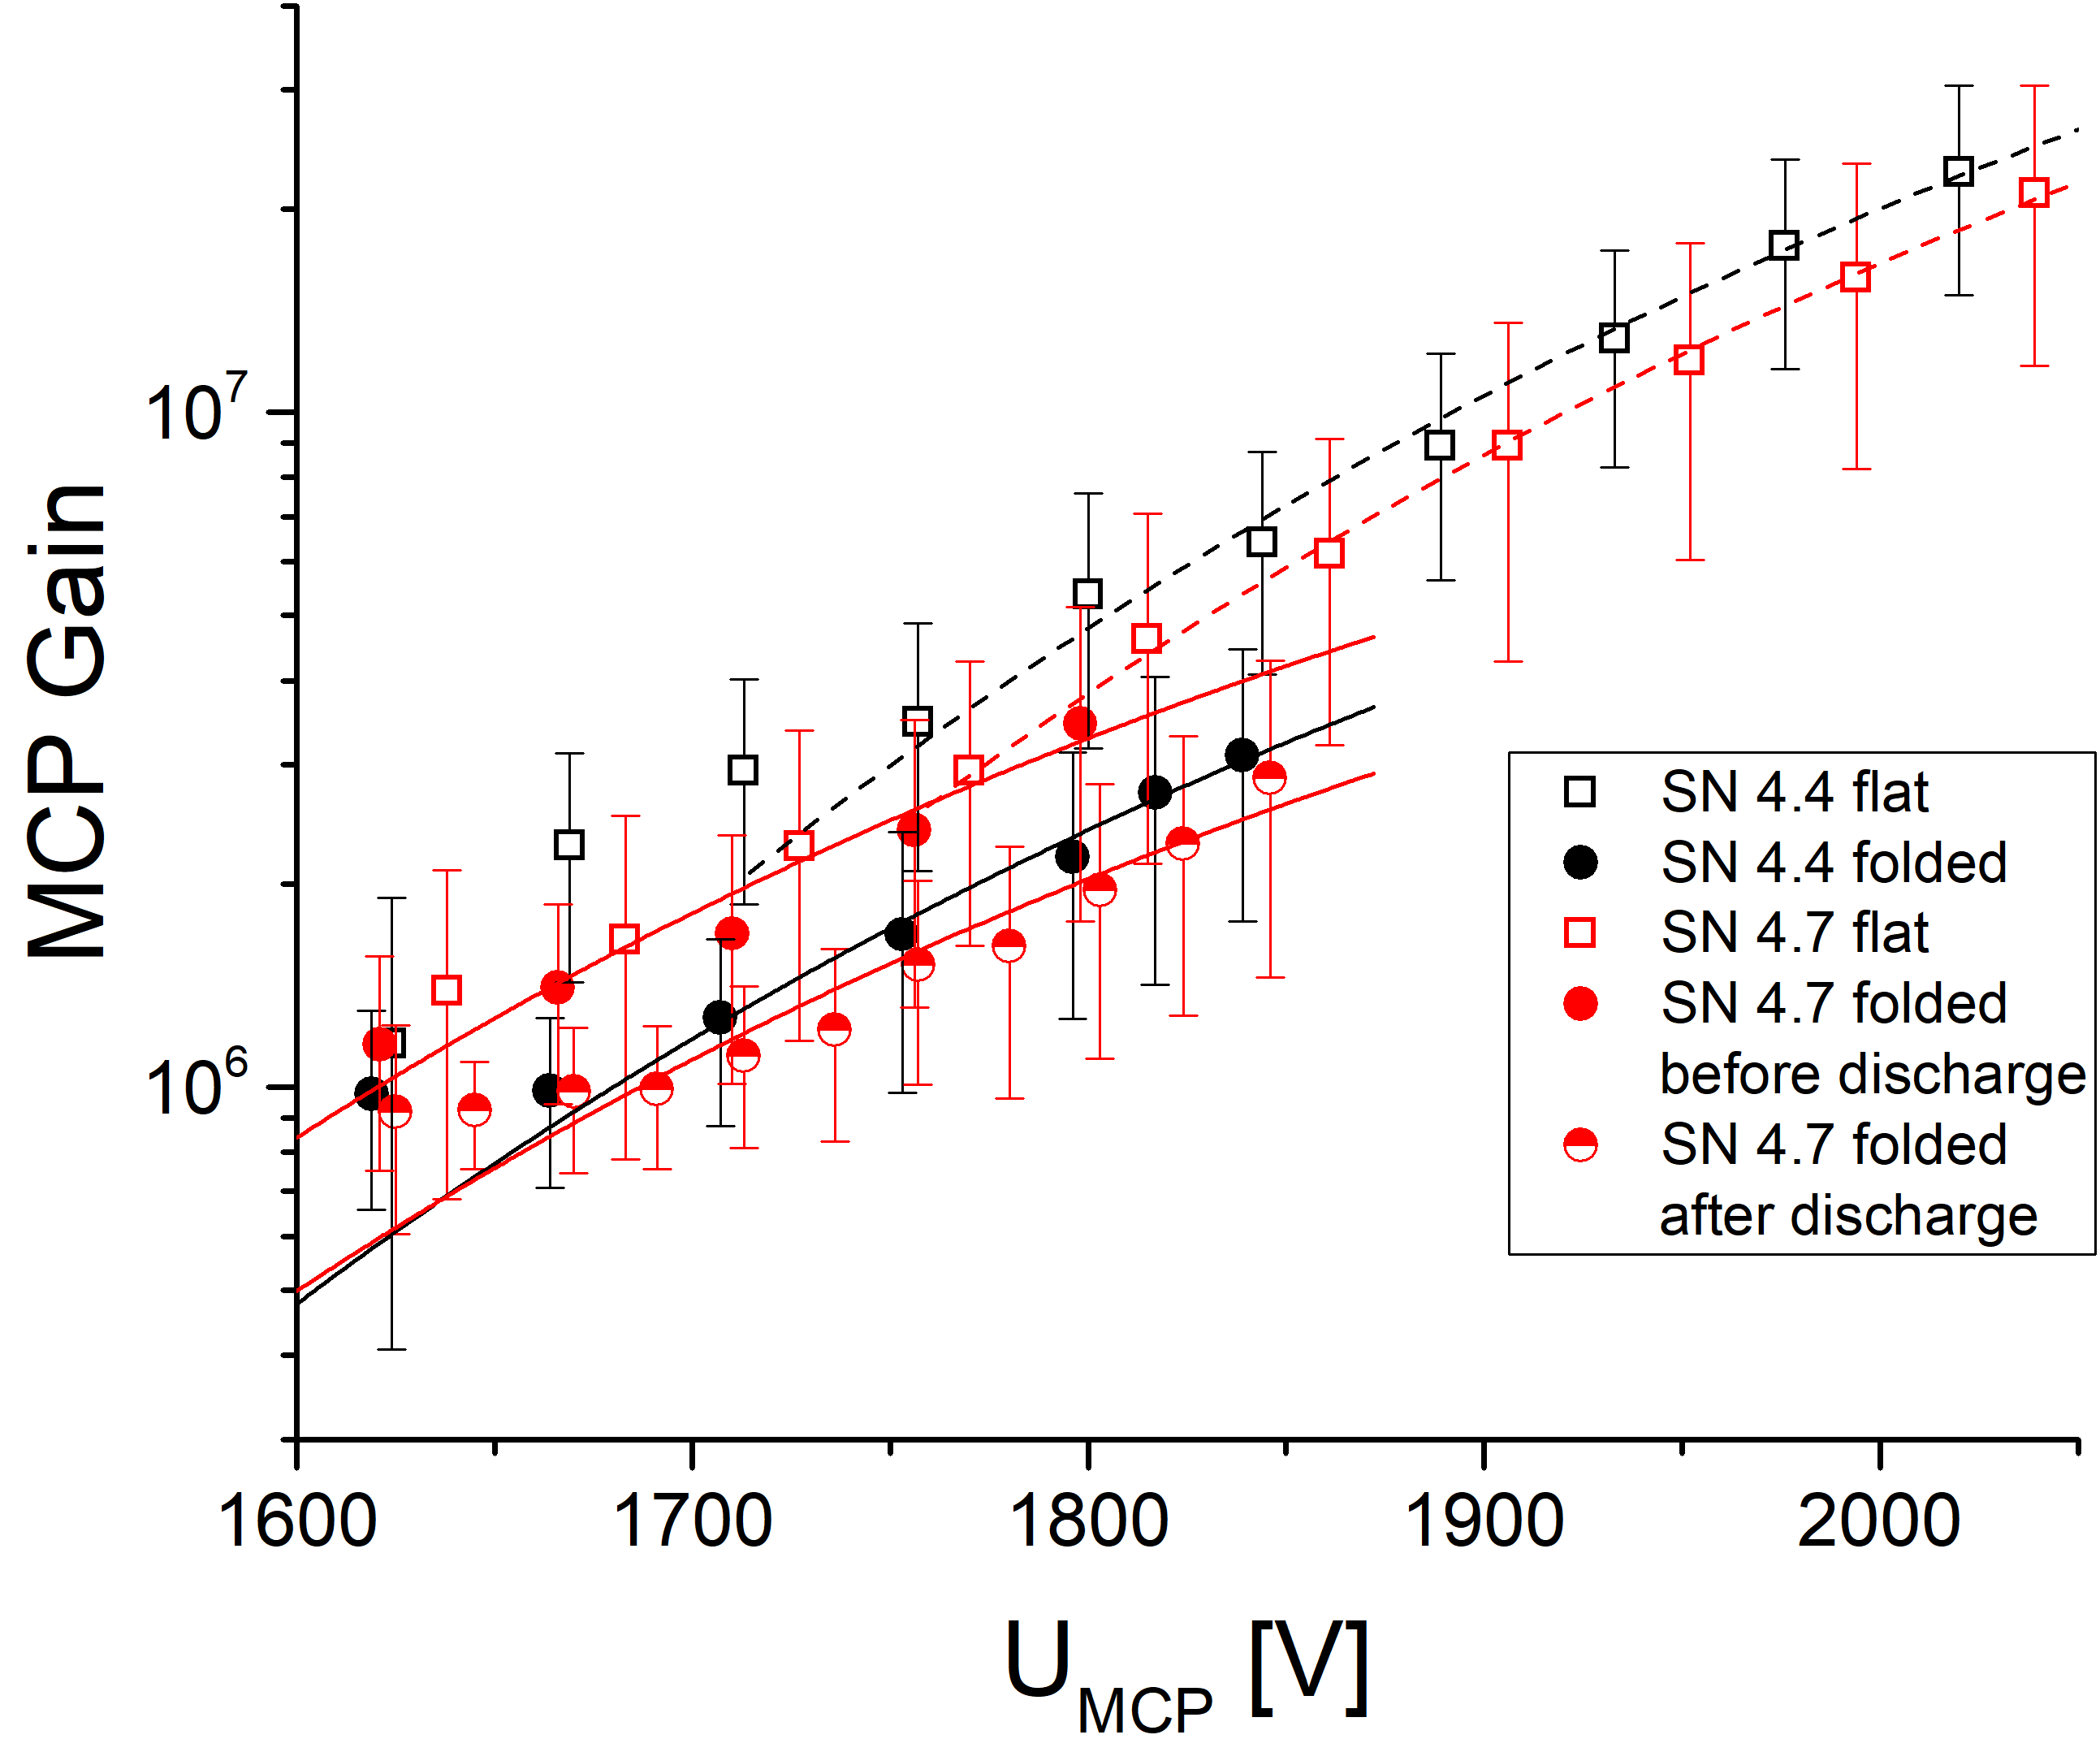
\includegraphics[width=0.9\textwidth]{Bilder/Gain_Curves_SN4p5_4p7.png}
		\end{subfigure}
		\begin{subfigure}{.5\textwidth}
			\centering
			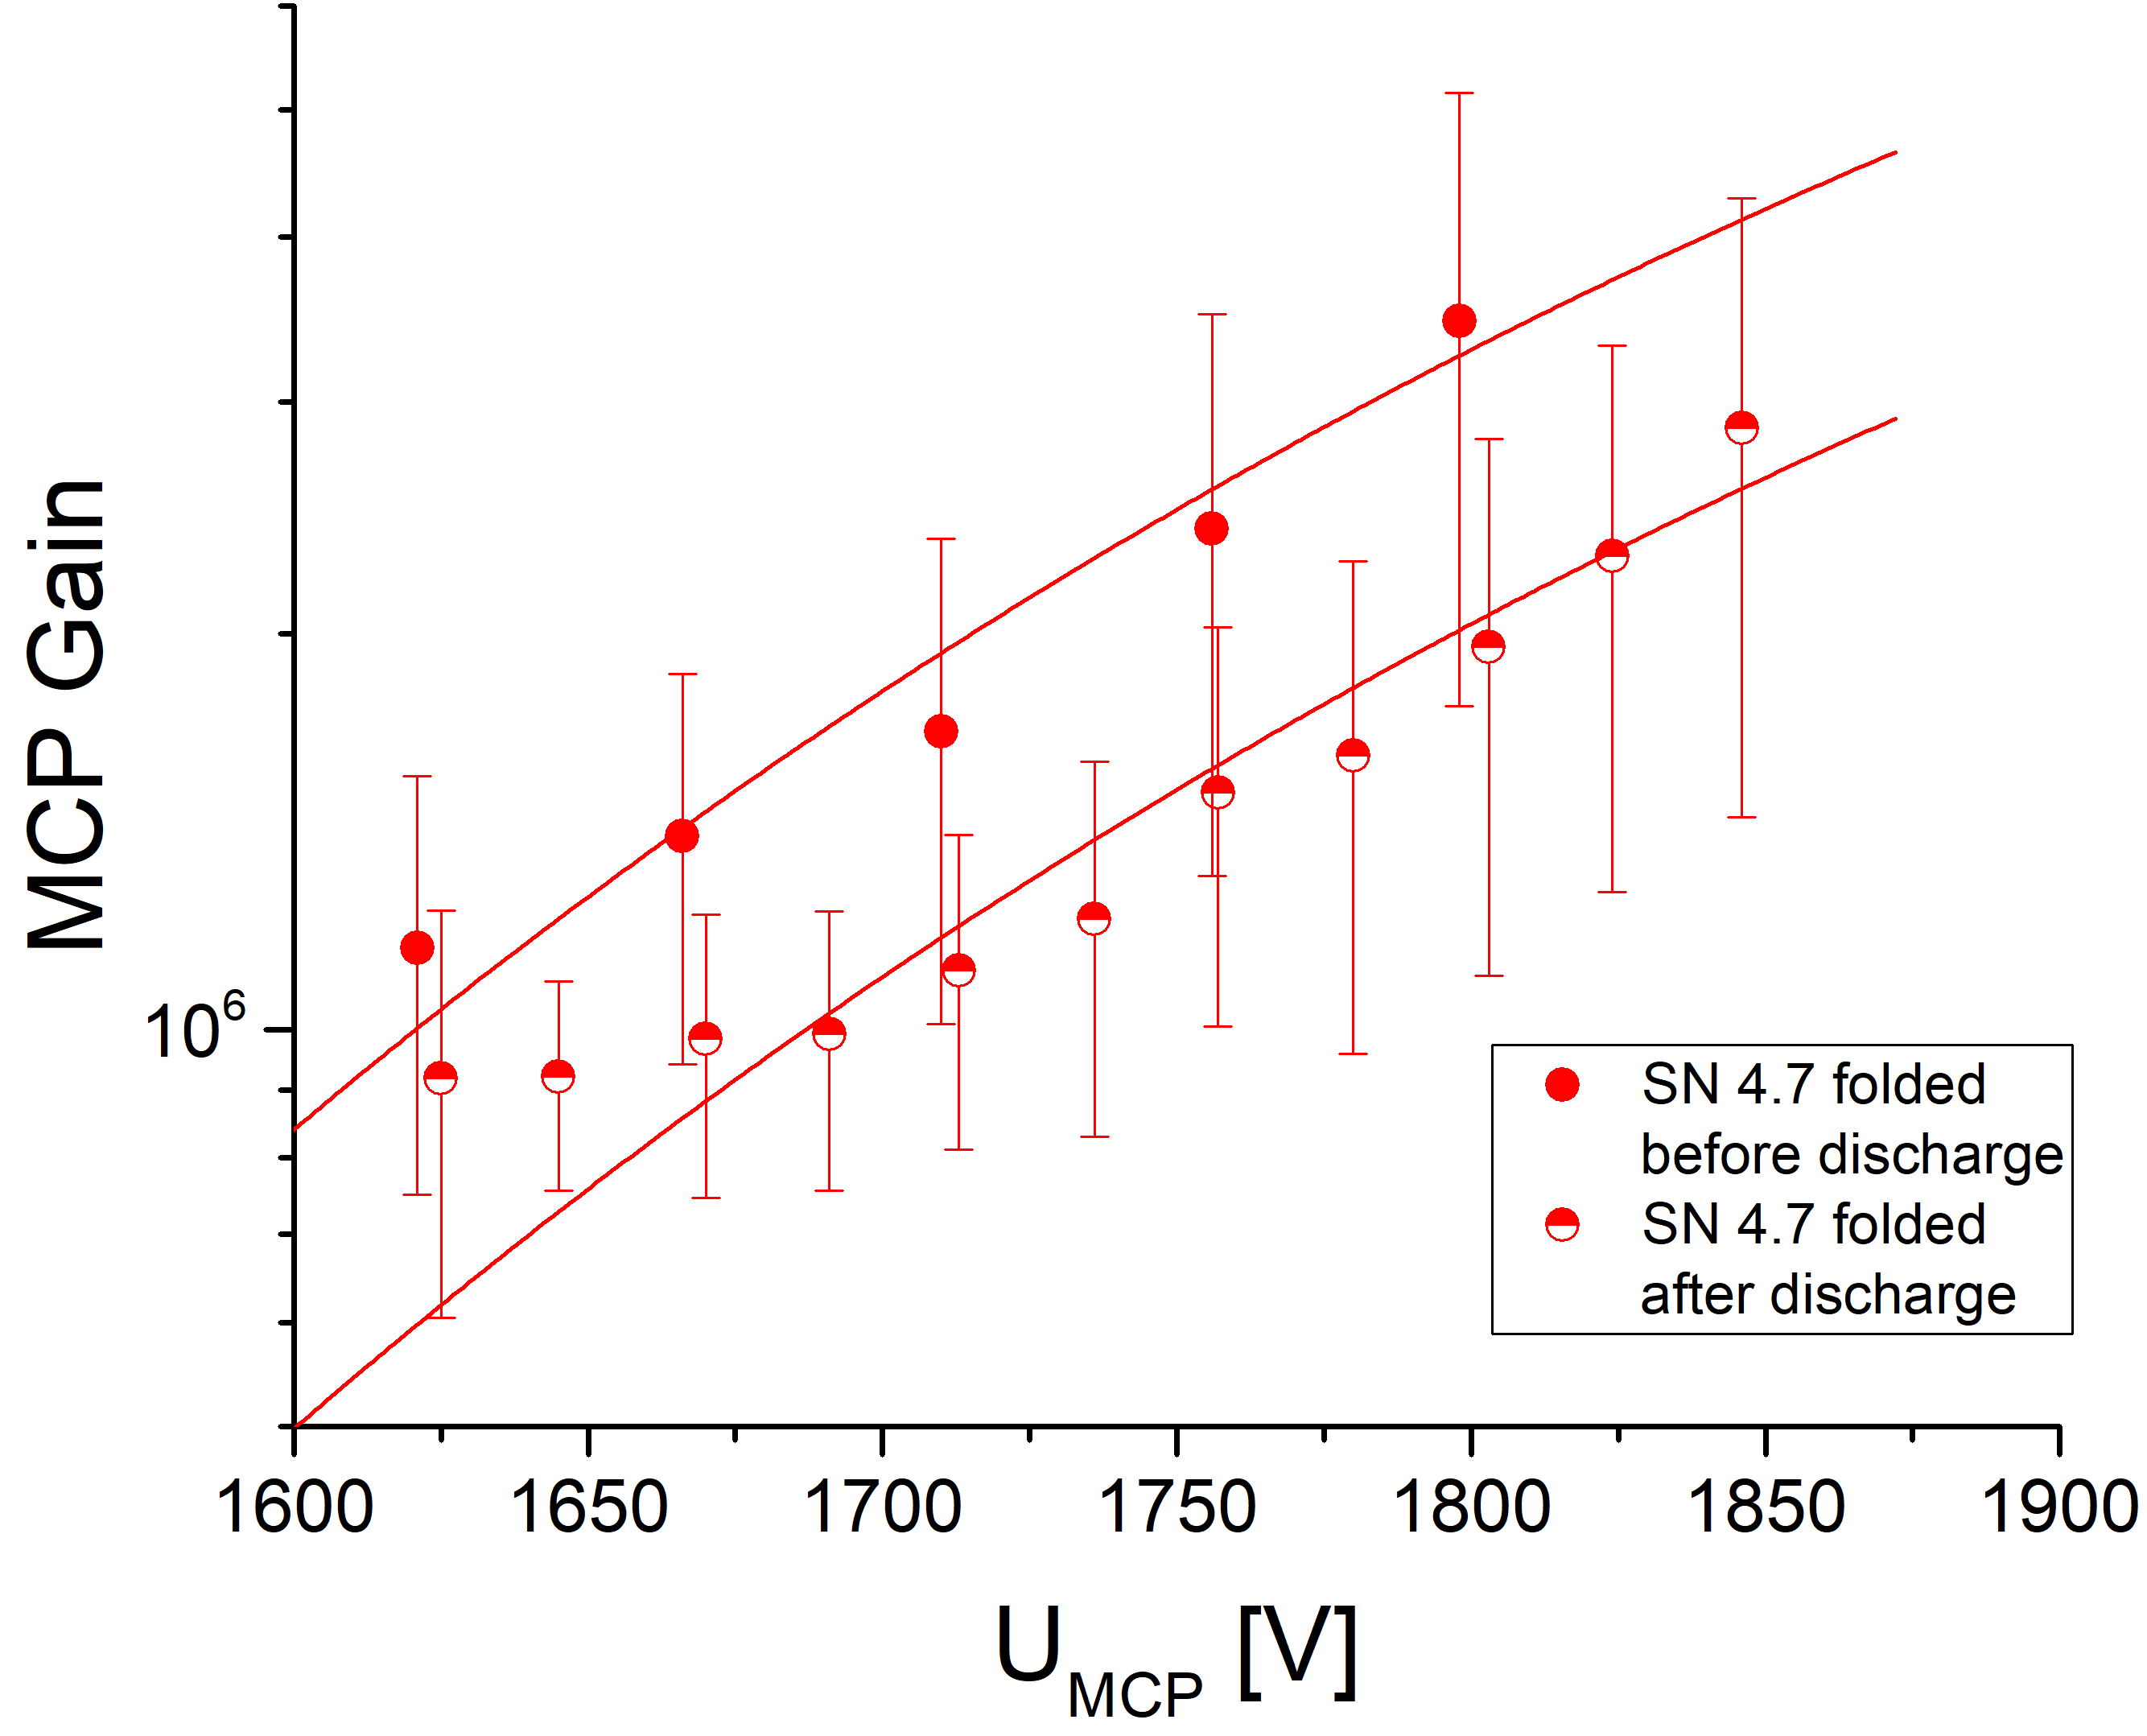
\includegraphics[width=0.9\textwidth]{Bilder/SN4p7_discharge.png}
		\end{subfigure}
		\caption{Left: Gain curves of two NIM PFM detectors. The difference in gain is because for each measurement curve, a different set of MCPs was used. Right: Gain curves of a folded NIM PFM detector. The lower gain curve was recorded after a discharge at an MCP voltage of 1.8\si{\kilo\volt}.}
		\label{fig:SN4p54p7Gain}
	\end{figure}
	% Discussion about the discharge behaviour in regards to gain. Are there any values? Something with free electrons destroying the inner coating of the MCP channels. Only a rough estimate needed.
	% Explanation of the fit model in theory part. -> Maike if there is any theory about that topic specifically.	
	
	% ROSETTA? When was a resistor latest used? Have a look if there is a space for sort of improvements of the sensor. If it is part of the experiments of of the thery part...
	% Explain, which measurements were made with which MCPs, describe how the discharge influences the signal. How much of the signal we loose in this specific measurement. Literature references?
	% Description of the current measurement of the detector with the laboratory electronics attached and then the calculation of the MCP voltage. State clearly under with circumstances the calculation with this method is possible and under which it is not (ion current, which is falsely taken into account)
	% Precise can we estimate the numbr of ions/ the partial pressure of the gas?
	% Describe, how far we tried to approximate the voltage.
	
	% Plot off the gain curves of the detector in its different states. flat, folded, folded in the wolfram copper shealding.
	% Measuring settings. Turn the drift voltage up to -2.5 kV and then slowly increase the anode voltage to the value you want to measure. The gain is calculated with the software by doing a Simpson 3/8 integration of the peak = Q. (Look in the lab book for the proper calculation)
	% Maybe there is time to redo the tests with the real PFM detector (XD wär schön. Leider nein). (Die Resultate sind nicht so vollständig wie die von der einen anderen Messung. Messung mit einem Zwillingsdetektor und von diesem auf den Flugdetektor schliessen. -> evt. schöne Graphik).
	
	
%-----------------------------------------------------------------------------------
	\subsection{Ionoptics}
	\subsubsection{Voltage Optimisation}
	Two types of electrical lenses. positive and negative voltage lenses. positive and negative voltage lenses have the same effect. In negative voltage lenses, the particles fly faster = shorter time-of-flight. This results in a better mass resolution.\\
	Aim in the lab is to get two different voltage sets. One for positive voltages to not stress the equipment and one with negative voltage lenses to reach the maximal performance of the instrument. -> Tests showed no significant better mass resolution. A more detailed data analysis has to be made. % data in folder: \\titania\UserHomes\foehn\My Documents\PhD\Messungen\PFM\CASYMIR-C\nMode_voltageSet_Comparison_200430 
	
	\subsection{Instrument performance tests}
		% At the end, make a comparison of the discussion of the different instruments as mass resolution, SNR as far as possible.
		\subsubsection{Prototype} % Final results. Only shpw best mass resolution achieved. May revere to Stefan's Diss. With the Prototype there were mainly componenets tests. Only discussion of the antechamber performance if it is not discussed in the chapter above.
		\subsubsection{PFM} % Include here the paper because it give a very good overview over the results conducted with it.
		\subsubsection{FS} % Include here the final results of the FS of this year with lab and flight electronics. Discussion about that subject, see PFM paper.
		% Laboratory and flight electronics are part of the same chapter because with the fligh electronics the only thing worth to discuss is the mass resolution because the signal intensity is still very low. Discuss the SNR graphics with Peter and then finalize this part of the chapter.
		
		% Look up the conditions for the description.
		\textbf{Ion Storage two different velocities}\\ % Ref. to Abplanalp paper.
		Ion storage is very crucial for a time of flight mass spectrometer because every ion generated and not stored in the ion source is lost and can generate additional electrical noise on the detector signal line. In this test the ion storage behaviour of the ion source was analysed for thermal and neutral mode for hydrogen and krypton with velocities of 2\,\si{\kilo\meter\per\second} and 4\,\si{\kilo\meter\per\second}. The emission current was varied from 20 to 600\,\si{\micro\ampere}. Ion storage of positive ions in x- and y- direction is supported by the negative potential generated by the electron beam. Two ring electrodes with a positive voltage applied generate a positive potential ring to trap generated ions in y- and z- direction (Fig.\ref{fig:ExpFSFlightSenIonStorIS}). For emission currents from 20 to 600\,\si{\micro\ampere} according to Eq.\,\eqref{eq:elPotIem} the negative potential in the centre of the electron beam is -0.08-(-2.59)\,\si{\volt}. Fig.\ref{fig:ExpFSFlightSenIonStor} left shows the ion storage behaviour of the ion source of hydrogen and right the ion storage behaviour of krypton. In case of no ion storage, the relationship between the electron emission current I\textsubscript{em} and the signal intensity is linear. In case of ion storage there is a quadratic relationship between I\textsubscript{em} and the signal intensity. When measuring with the thermal mode, the particles get slowed down until they have energies in the range of 0.01\,\si{\electronvolt} and are therefore easy to trap in the potential field. In neutral mode particles enter the ionisation region directly. The kinetic energy of hydrogen for velocities between 2-4\,\si{\kilo\metre\per\sec} is 0.07-0.27\,\si{\electronvolt}. It can therefore easy be trapped in the potential field by the electron beam and the potential of the ring electrode already with very emission currents as low as 20\,\si{\micro\ampere}.\\
		The kinetic energy of \textsuperscript{84}Kr for the same velocities is 2.8-11.2\,\si{\electronvolt}. This energy exceeds the potential of the centre of the electron beam and the ions are therefore more difficult to trap with only the electron beam. The ions are kept in the middle of the ionisation region with the positive potential ring. According to Fig.\,\ref{fig:ExpFSFlightSenIonStor} ion storage for \textsuperscript{84}Kr starts to dominate at emission currents of 100\,\si{\micro\ampere}.
		%Therefore there is no difference in the measured intensities for hydrogen when it enters with 2 or 4\,\si{\kilo\meter\per\second}.\\		
		In thermal mode, an increase in beam velocity leads to an increase in signal intensity due to the density enhancement effect \textcolor{red}{(Ref.)}. Therefore a higher signal intensity is expected in thermal mode for 4\,\si{\kilo\meter\per\second} compared to 2\,\si{\kilo\meter\per\second}. 
		Like the in PFM, the FS shows a nice ion storage behaviour. For krypton ion storage just starts at an emission current of 100\,\si{\micro\ampere} where hydrogen is stored already at lower emission currents due its lower kinetic energy at the same beam velocity.
		
		\begin{figure}[h]
			\centering
			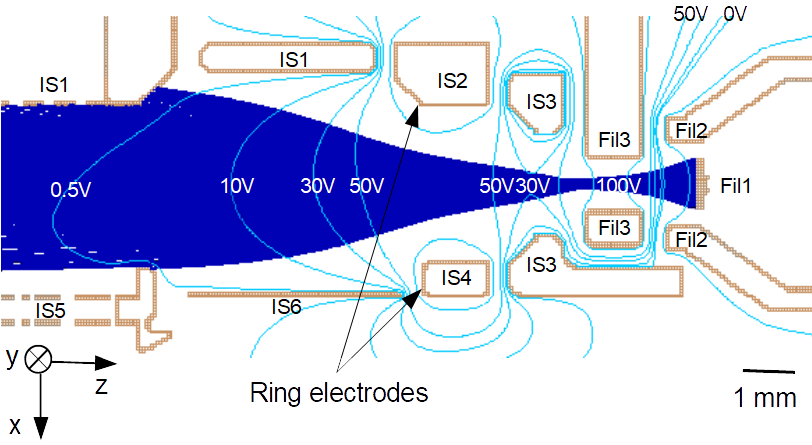
\includegraphics[width = 0.8\textwidth]{Experiments/FiL_IS_elBeam_Storage.png}
			\caption{Ion storage source with sample voltage set applied to the electrodes. In light blue are the potential lines and in dark blue a simulated electron beam.}
			\label{fig:ExpFSFlightSenIonStorIS}
		\end{figure}
		
		
		\begin{figure}[h] % Ion storage. Exchange Graphics as soon as discussed with Peter how to proper show the results.
			\begin{subfigure}{0.5\textwidth}
				\centering
				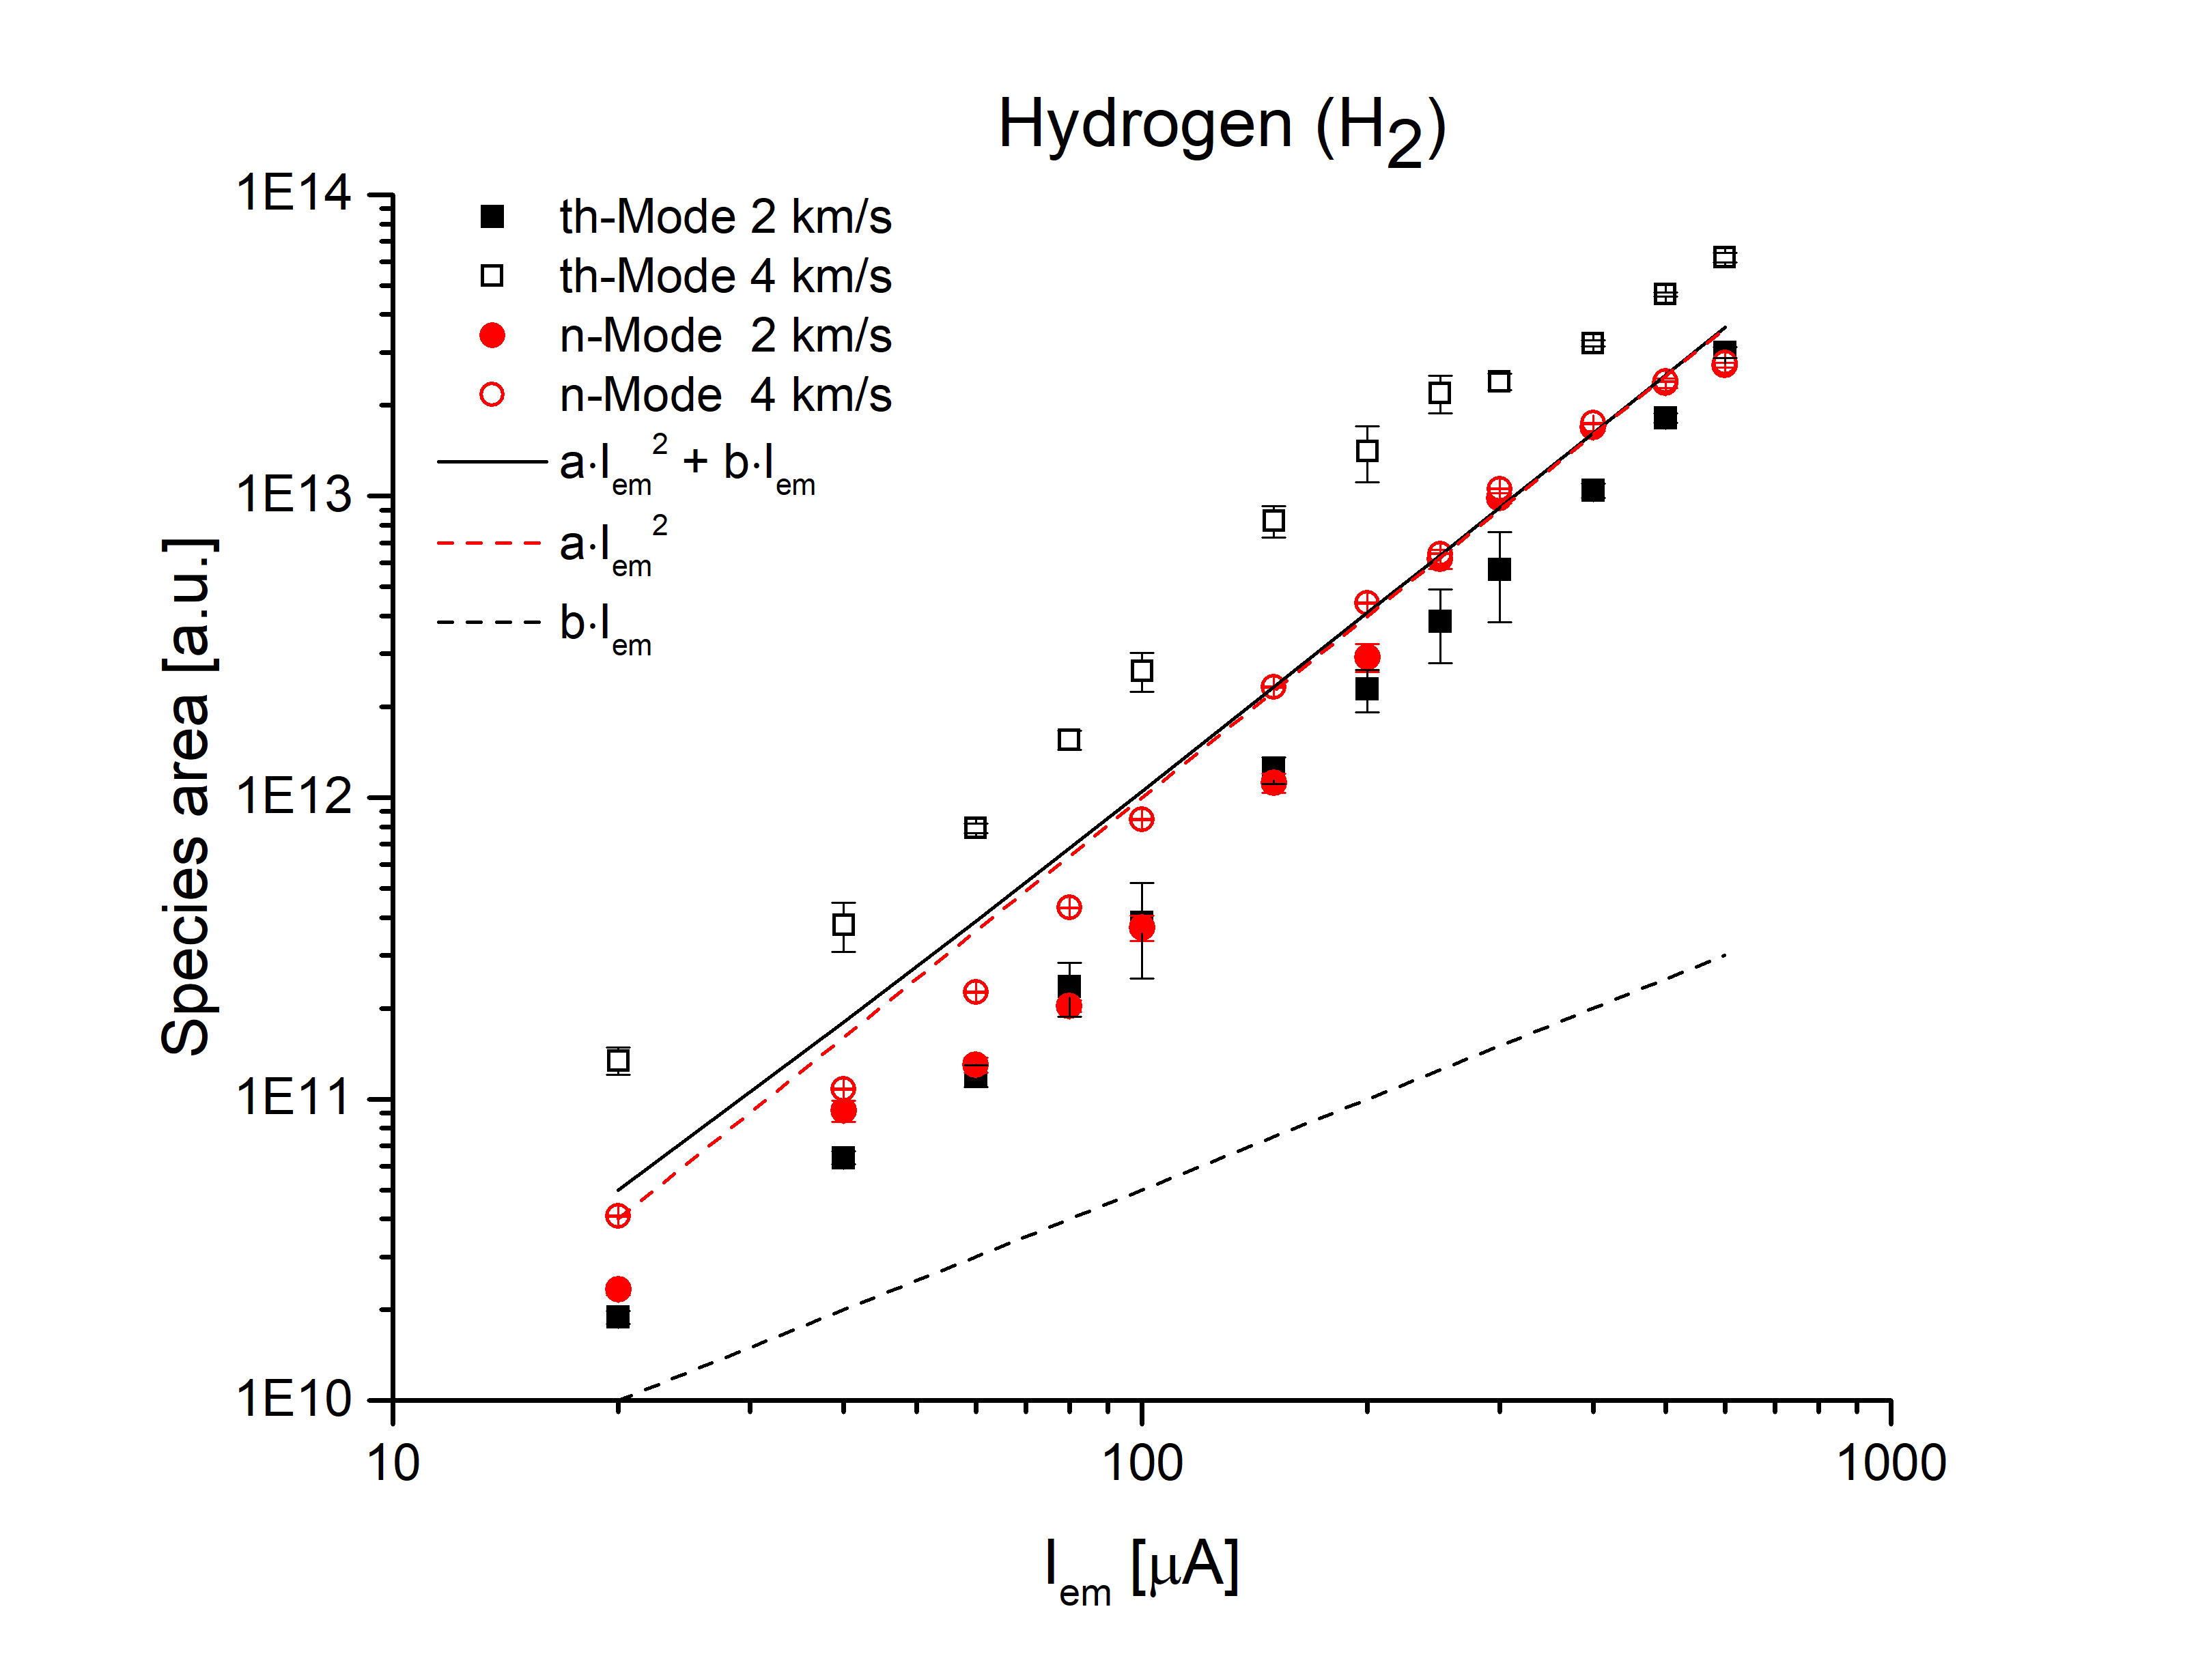
\includegraphics[width = \textwidth]{Experiments/FSLabIonStorageH2.png}
			\end{subfigure}
			\begin{subfigure}{0.5\textwidth}
				\centering
				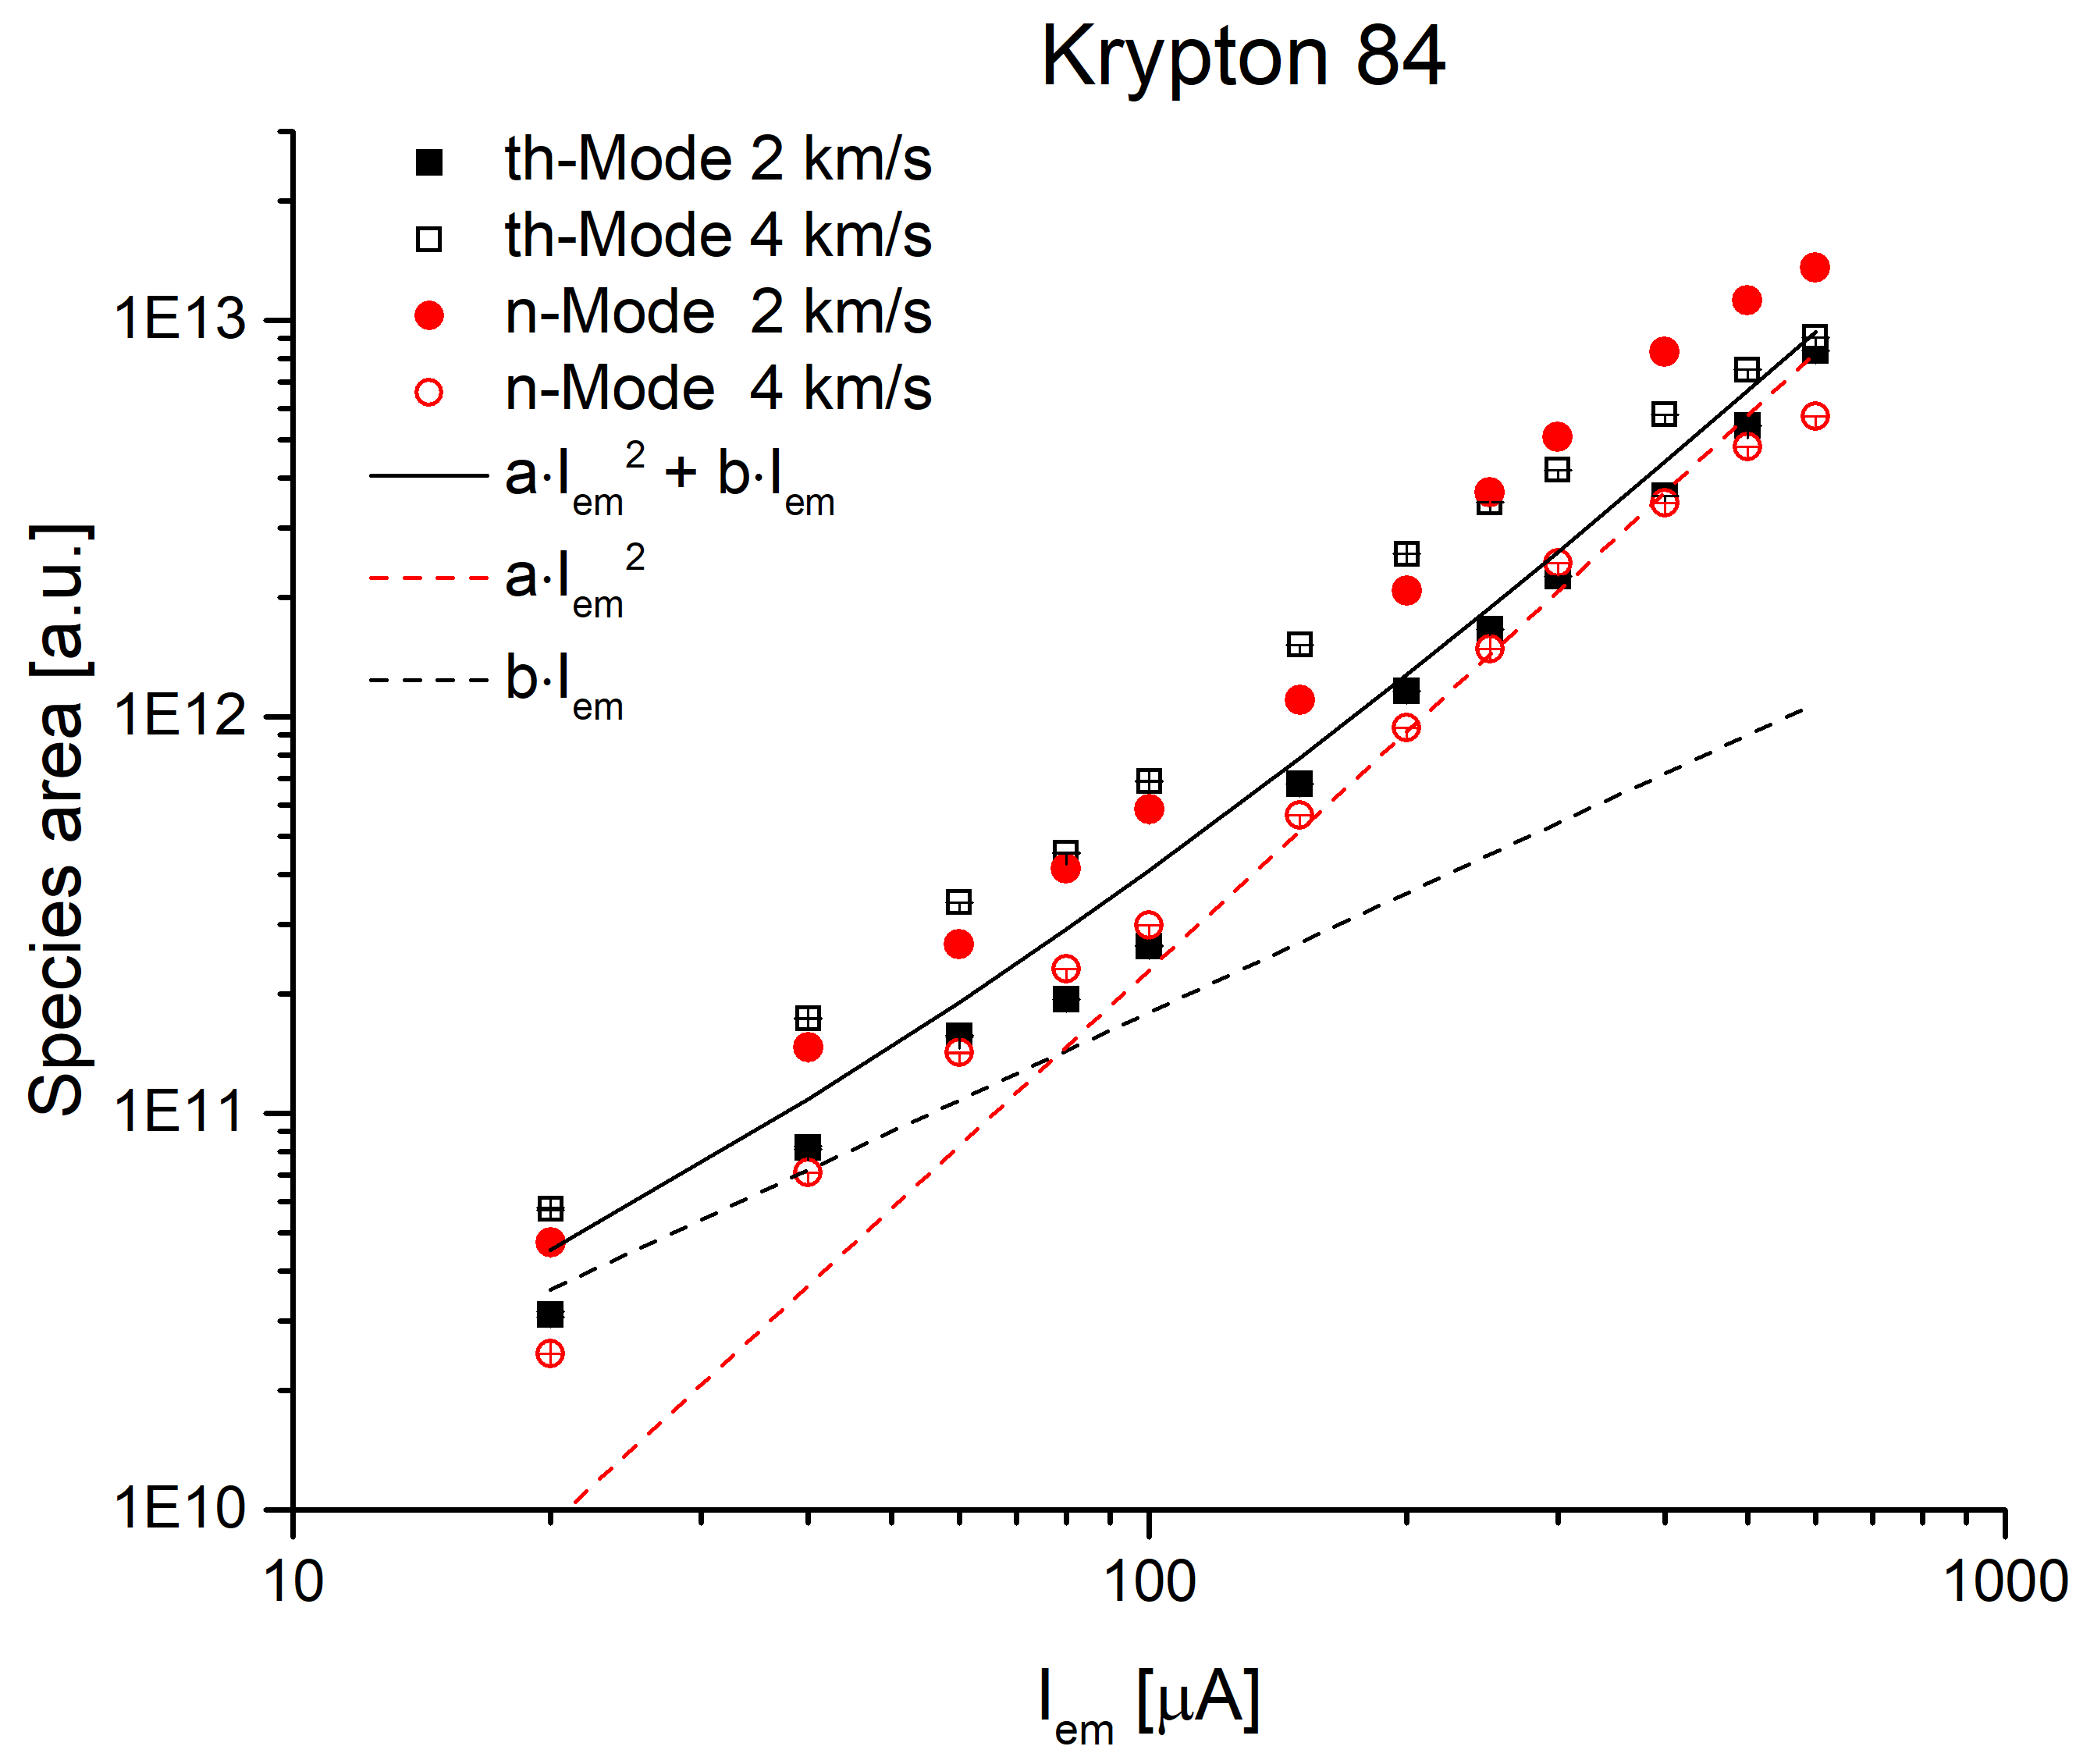
\includegraphics[width = \textwidth]{Experiments/FSLabIonStorageKr84.png}
			\end{subfigure}
			\caption{Ion storage measurement with the flight spare sensor but with laboratory electronics attached for H$_2$ and $^{84}$Kr for two different gas velocities.}
			\label{fig:ExpFSFlightSenIonStor}
		\end{figure}

		% Detector behaviour test in FS sensor. Formula derivation is in the theory part with the proper detrivation.
		% No saturation observed. 

		\textbf{Mass resolution and Signal-to-Noise Ratio}\\
		According to the requirements stated in (Ref.) % See paper
		the required mass resolution for neutral mode is 500 and for thermal mode it is 1000 m/dm but to be able to distinguish between different masses at unit masses of 1000\,u NIM has to have a mass resolution of 1000. Otherwise NIM the different unit masses cannot be distinguished. Fig.\,\ref{fig:ExpFSFlightSenMassRes} show two spectra recorded with the NIM flight sensor with laboratory electronics attached with an electron emission current of 100\,\si{\micro\ampere}. With a mass resolution of 708 for neutral gas mode NIM fulfils the requirements. In thermal gas mode the highest mass resolution achieved was 830 m/$\Delta$m which comes close to the requirements. Fig.\,\ref{fig:ExpFSFlightElMassRes} show the mass spectra recorded with the NIM flight sensor with the flight electronics attached. The electron emission current was 200\,\si{\micro\ampere} the highest mass resolution achieved at the current state is 490 m/$\Delta$m for neutral gas mode and 462 m/$\Delta$m for thermal mode. Fig.\,\ref{fig:ExpFSFlightElK78} shows a mass spectrum recorded in thermal mode with an emission current of 300\,\si{\micro\ampere} the $^{78}$Kr peak is clearly visible. The signal to noise ratio for the spectra recorded with the flight electronics is very low compared to the SNR for the spectra recorded with the laboratory electronics. We also observe noisy part wandering between the single spectra. There is a significant part of repetitive noise appearing not always at the same position in the spectrum. With a proper noise filter this noise can be detected and significantly reduced without affecting the mass signal peaks. For future work, there is a lot of potential for improving the spectrum by proper analysing the noise and writing filters to suppress the noise.\\
		Fig.\,\ref{fig:ExpFSFlightSenSNR} shows a mass spectrum recorded with the flight sensor with the laboratory electronics attached. The highest SNR achieved was $6\cdot10^{5}$ and therefore almost 6 decades. % Explanation why the 6 decades are required.
		The mass peaks 355\,u, 390\,u and 429\,u are some oil components with water adducts coming from the used turbo pumps of the test facility. 415\,u is an artefact coming from the background subtraction algorithm. The artefact peak is also wider then the other surrounding mass peaks.
		
		\begin{figure}[h]
			\begin{subfigure}{0.5\textwidth}
				\centering
				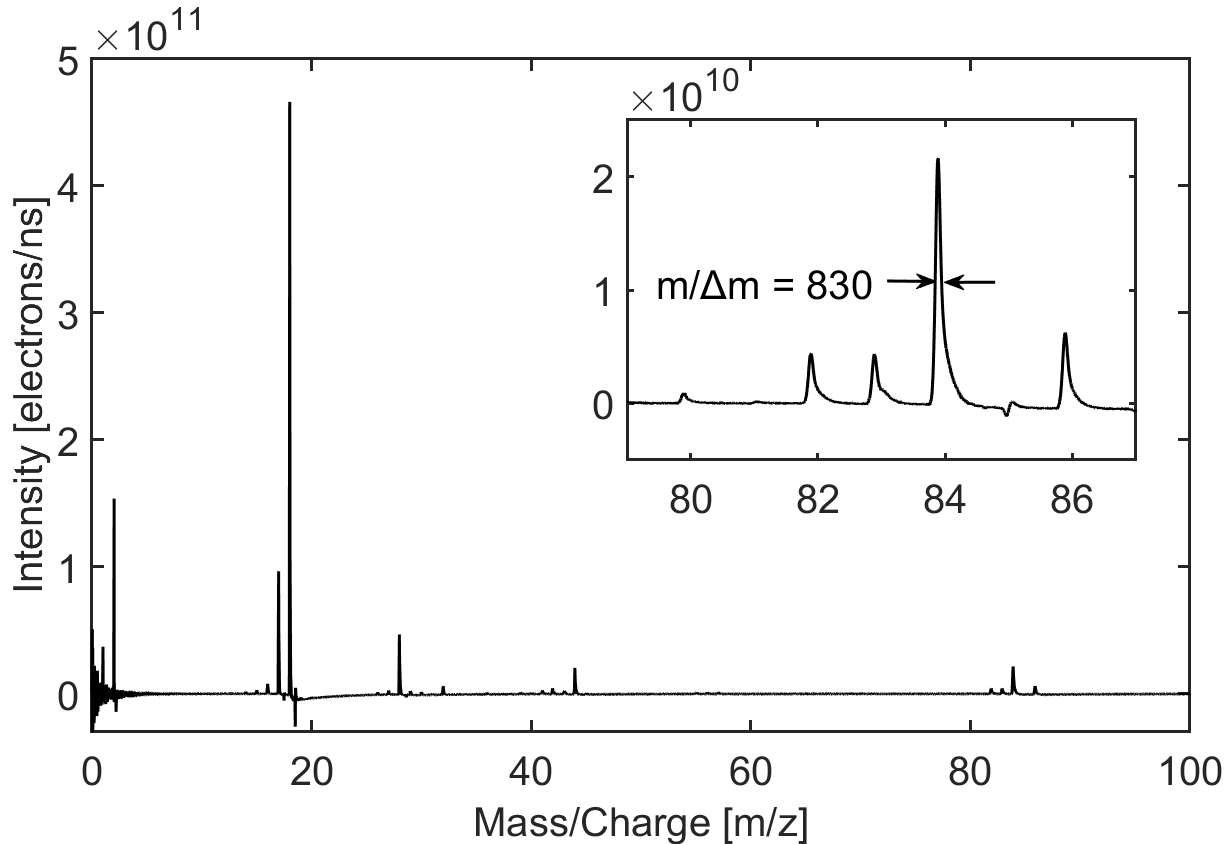
\includegraphics[width = \textwidth]{Experiments/FSLabthMode.png}
			\end{subfigure}
			\begin{subfigure}{0.5\textwidth}
				\centering
				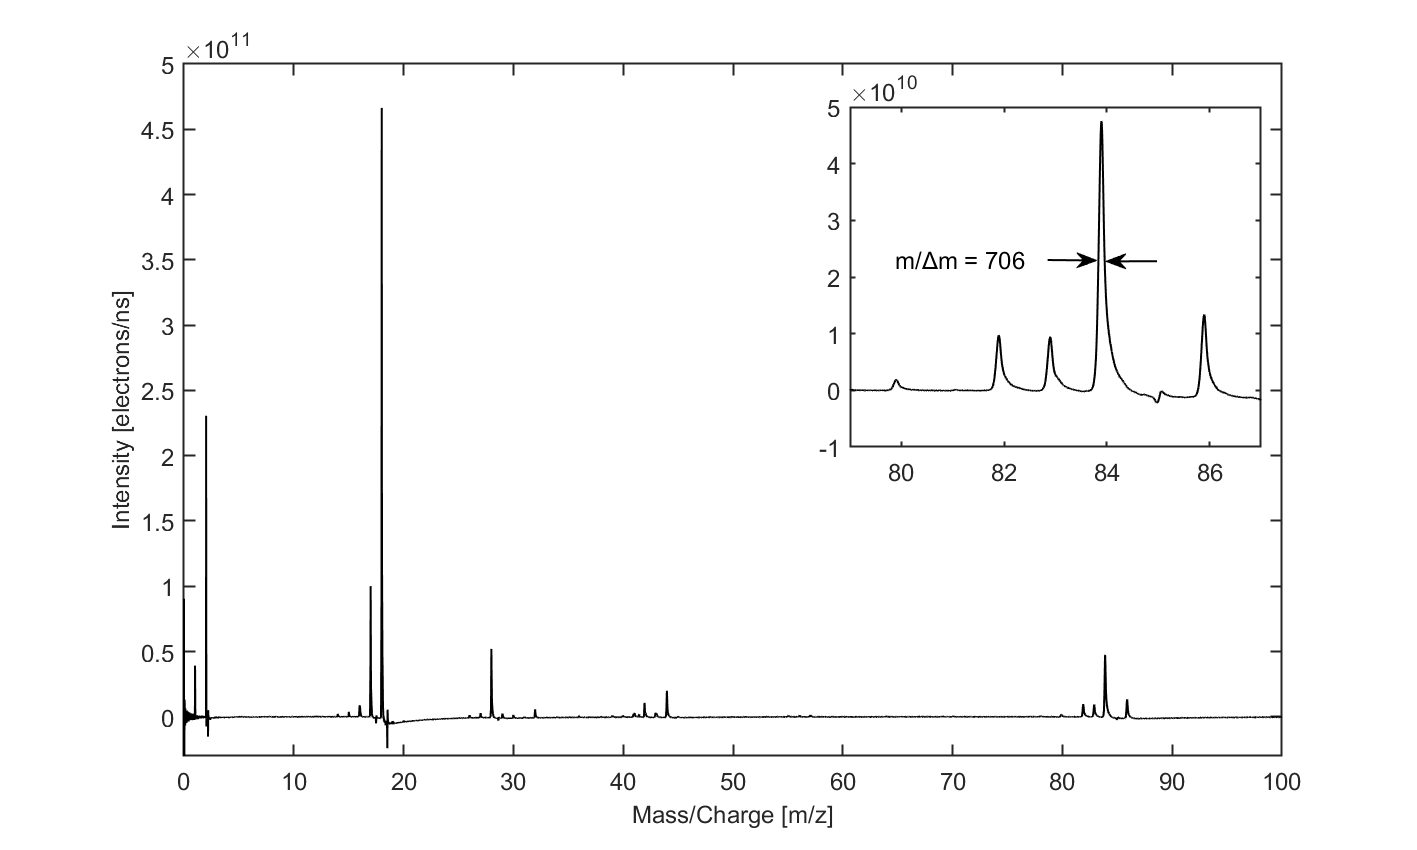
\includegraphics[width = \textwidth]{Experiments/FSLabnMode.png}
			\end{subfigure}
			\caption{Mass spectra measured with the flight spare sensor with the laboratory electronics electronics attached. Left: with thermal gas mode Right: neutral mode.}
			\label{fig:ExpFSFlightSenMassRes}
		\end{figure}

		% Mark the noisy part for better description to explain that
		% conditions: nMode UMCP: 1950 V. P = 1.03e-8 mbar 20H2:1Kr
		%			thMode UMCP = 1950 V. P = 6.05e-8 mbar
		\begin{figure}[h]
			\begin{subfigure}{0.5\textwidth}
				\centering
				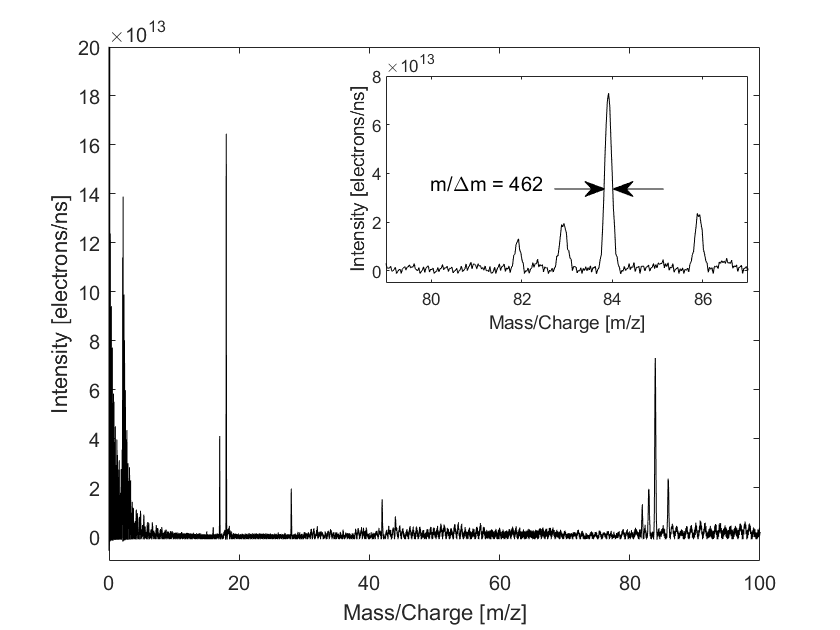
\includegraphics[width = \textwidth]{Experiments/FSthMode200uA.png}
			\end{subfigure}
			\begin{subfigure}{0.5\textwidth}
				\centering
				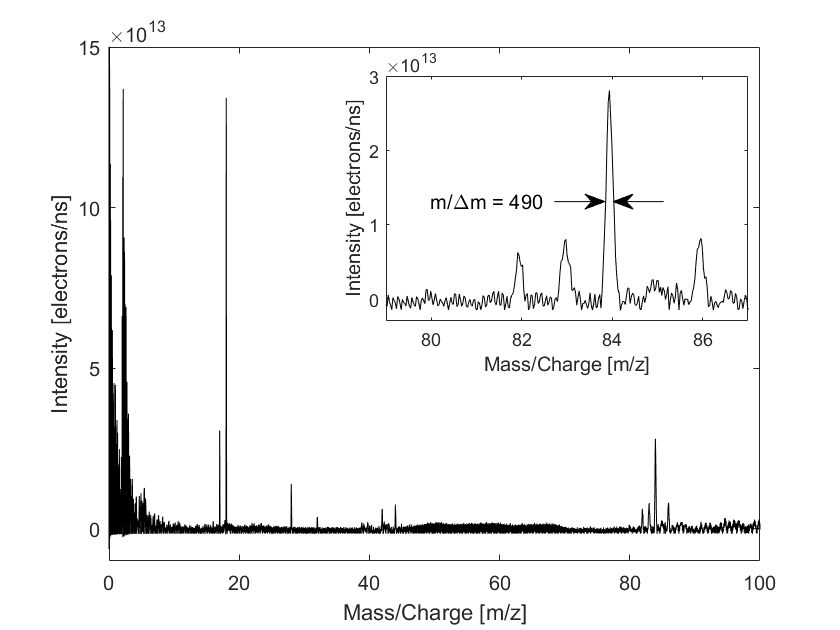
\includegraphics[width = \textwidth]{Experiments/FSnMode200uA.png}
			\end{subfigure}
			\caption{Mass spectra measured with the flight spare instrument with the flight electronics attached. Filament emission current was 200 \si{\micro\ampere}. Left: with thermal gas mode Right: neutral mode.}
			\label{fig:ExpFSFlightElMassRes}
		\end{figure}
		
		\begin{figure} % Point out at that picture that the Kr 78 isotope is clearly visible.
			\centering
			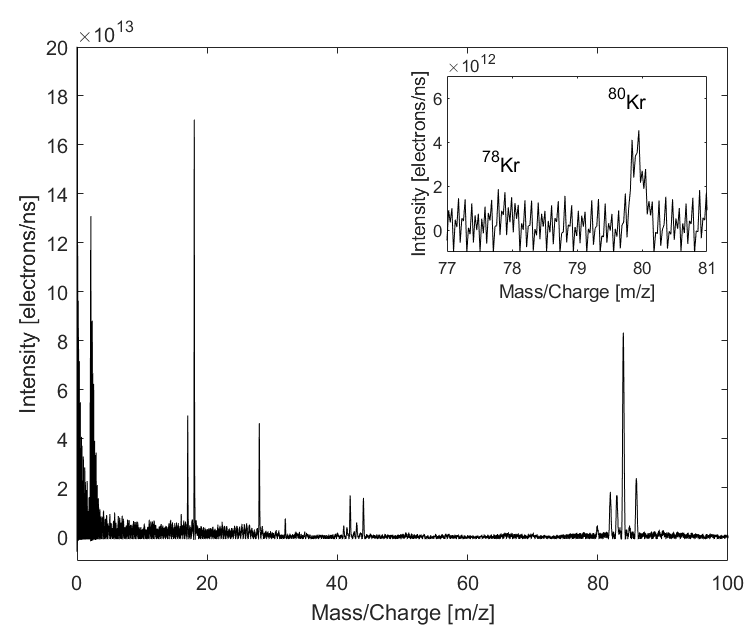
\includegraphics[width = 0.6\textwidth]{Experiments/FS_thMode300uA.png}
			\caption{Mass spectra measured with the flight spare instrument with the flight electronics attached. Filament emission current was 300 \si{\micro\ampere}.}
			\label{fig:ExpFSFlightElK78}
		\end{figure}
		
		% SNR 600 uA emission current. Rest gas Ptot = 1.6e-9 mbar, UMCPeff = 1.8 kV. Name the gas peaks. Peaks around 200 u are not mercury because the isotopic ratio does not match the pattern.
		\begin{figure}[h]
			\centering
			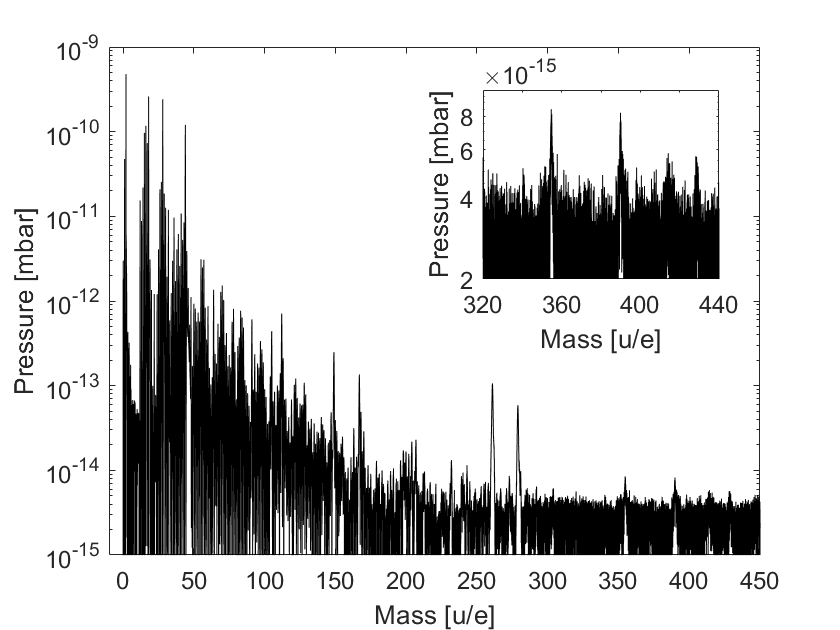
\includegraphics[width = 0.7\textwidth]{Experiments/FSLabSNRRestGasPressCal.png}
			\caption{SNR plot for the flight spare sensor but with laboratory electronics attached at a chamber pressure of 1.5$\cdot10^{-9}$\si{\milli\bar}.}
			\label{fig:ExpFSFlightSenSNR}
		\end{figure}
	
	
	
	
	
	
	